\documentclass[useAMS,usenatbib]{mn2e}
\usepackage[toc,page]{appendix}
\usepackage{natbib}
\usepackage{amssymb}
\usepackage{epsf}
\usepackage{pstricks}
\usepackage{color}
\usepackage{graphicx}
\usepackage{slashed}
\usepackage{relsize}
\usepackage{morefloats}
\usepackage{multirow}

%\usepackage {amsmath}
%\usepackage {amsxtra}
%\usepackage {amsbsy}
%\usepackage {amscd}
\usepackage {array}

%\usepackage {graphics}
%\usepackage {amsfonts}
%\usepackage {float}
%\usepackage {indentfirst}
%\usepackage{verbatim}

%\usepackage {a4wide}
%\usepackage {setspace}
%\usepackage{enumitem}
\usepackage{hyperref}
%\usepackage[all]{hypcap}
%\usepackage{caption}
\usepackage[justification=centering]{caption}

\newcommand{\nat}{Nature}
\newcommand{\mnras}{MNRAS}
\newcommand{\apj}{ApJ}
\newcommand{\apjl}{ApJL}
\newcommand{\apjs}{ApJS}
\newcommand{\aap}{A\&A}
\newcommand{\pasa}{PASA}
\newcommand{\apss}{ApSS}
\newcommand{\araa}{ARAA}
\newcommand{\aj}{Astron. J.}
\newcommand{\aaps}{A\&AS}
\newcommand{\aplett}{Astrophys. Lett.}

%\topmargin=-0.4in

%%%%%%%%%%%%%%%%%%%%%%%%%%%%%%%%%%%%%%%%%%%%%%%%%%%%%%%%%%%%%%%%%%%%%%
\bibliographystyle{mn2e}
\begin{document}

\title[A Study of the Multi-frequency Polarization Pulse Profiles of Millisecond Pulsars]{A Study of the Multi-frequency Polarization Pulse Profiles of Millisecond Pulsars}
\author[S. Dai et al.]{S. Dai$^{1,2}$, G. Hobbs$^1$, M. Kerr$^1$, R. N. Manchester$^1$, R. Shannon$^1$, M. Bailes$^3$,  
\newauthor N. D. R. Bhat$^4$, S. Burke-Spolaor$^5$, W. A. Coles$^6$, M. J. Keith$^7$, Y. Levin$^8$, A. Mata$^9$,
\newauthor S. Os\l owski$^{10,11}$, V. Ravi$^{12}$, J. M. Sarkissian$^{13}$, C. Tiburzi$^{14,15,1}$, L. Toomey$^{1}$, 
\newauthor W. van Straten$^3$, H. G. Wang$^{16,1}$, J.-B. Wang$^{17}$, L. Wen$^{18}$, R. X. Xu$^2$, X.-J. Zhu$^{18}$\\
$^1$CSIRO Astronomy and Space Science, Australia Telescope National Facility, Box 76 Epping NSW 1710, Australia\\
$^2$Department of Astronomy, School of Physics, Peking University, Beijing 100871, China\\
$^3$Centre for Astrophysics and Supercomputing, Swinburne University of Technology, PO Box 218, Hawthorn, VIC 3122, Australia\\
$^4$International Centre for Radio Astronomy Research, Curtin University, Bentley, WA 6102, Australia\\
$^5$Department of Astronomy, California Institute of Technology, Pasadena, CA 91125, USA\\
$^6$Department of Electrical and Computer Engineering, University of California, San Diego, La Jolla, CA 92093, USA\\
$^7$Jodrell Bank Centre for Astrophysics, University of Manchester, M13 9PL, UK\\
$^8$School of Physics, Monash University, PO Box 27 Clayton, VIC 3800, Australia\\
$^9$Center for Advanced Radio Astronomy, University of Texas, Rio Grande Valley, Brownsville, TX 78520, USA\\
$^{10}$Max-Planck-Institut f\"{u}r Radioastronomie, Auf dem H\"{u}gel 69, D-53121 Bonn, Germany\\
$^{11}$Department of Physics, Universit\"{a}t Bielefeld Universit\"{a}tsstr. 25 D-33615 Bielefeld, Germany\\
$^{12}$School of Physics, University of Melbourne, Parkville, VIC 3010, Australia\\
$^{13}$CSIRO Astronomy and Space Science, Parkes Observatory, Box 276, Parkes NSW 2870, Australia\\
$^{14}$INAF–Osservatorio Astronomico di Cagliari, Via della Scienza, I-09047 Selargius (CA), Italy\\
$^{15}$Dipartimento di Fisica, Universit\`a di Cagliari, Cittadella Universitaria, I-09042 Monserrato (CA), Italy\\
$^{16}$School of Physics and Electronic Engineering, Guangzhou University, 510006 Guangzhou, China\\
$^{17}$Xinjiang Astronomical Observatory, Chinese Academy of Sciences, 150 Science 1-Street, Urumqi, Xinjiang 830011, China\\
$^{18}$Department of Physics, University of Western Australia, Crawley, WA 6009, Australia\\
}

\maketitle

\begin{abstract}

We present high signal-to-noise ratio, multi-frequency polarization profiles 
for $24$ millisecond pulsars that are being observed as part of the Parkes 
Pulsar Timing Array (PPTA) project. 
%
The pulsars are observed in three bands, centered at $728$, $\sim1369$
and $3100$ MHz, using a dual-band $10\rm{cm}$/$50\rm{cm}$ receiver and the 
central beam of the $20\rm{cm}$ multibeam receiver. 
%
Data sets that have been carefully calibrated over several years are utilized, 
which allows us to study the components and evolution of profiles with 
frequency, and to show previously undetected profile features. 
%
At $1400$ MHz, compared with previous results, the overall pulse width increases 
by $\sim22$ per cent on average, and $17$ of the $24$ pulsars show emission over 
more than half of the pulse period.
%
The morphology of pulse profiles shows clear frequency evolution, but 
the pulse widths are relatively constant with frequency.
%
The phase-resolved spectral indices show structures following the components 
of pulse profiles and the values significantly deviate from the mean spectral index.
%
We do not see simple frequency evolution of the polarization parameters, but 
there is evidence that pre-cursors and post-cursors have higher fractional 
linear polarization.
%
%These results support theories that suggest millisecond pulsar emission 
%regions are wider, at least in terms of pulse longitude, than those of the 
%normal pulsars. 
%The magnetic field of millisecond pulsars could be much more complicated 
%than a dipolar structure.
%
%Polarization variations across the profiles are complex, and the observed 
%position angle variations are generally not in accord with the rotating vector 
%model for pulsar polarization. Nevertheless, the polarization properties are 
%broadly similar to those of normal (non-millisecond) pulsars, suggesting that 
%the basic radio emission mechanism is the same in both classes of pulsar.
%The results support the idea that radio emission from millisecond pulsars 
%originates high in the pulsar magnetosphere, probably close to the emission 
%regions for high-energy X-ray and gamma-ray emission. Rotation measures were 
%obtained for all 20 pulsars, eight of which had no previously published 
%measurements.


\end{abstract}



\begin{keywords}
%
pulsars: general
%
\end{keywords}


\section{Introduction}

Millisecond pulsars (MSPs) are a special subgroup of radio pulsars. 
%
Compared with ``normal'' pulsars, they have much shorter spin periods 
and smaller spin-down rates, and therefore have larger characteristic 
ages and weaker implied dipole magnetic fields.
%
The short spin periods and highly stable average pulse shapes of MSPs 
make them powerful tools to investigate various astrophysical phenomena 
using high precision timing of the pulse arrival times~\citep[e.g.,][]{Manchester08}.
%

The Parkes Pulsar Timing Array (PPTA) project (Manchester et al. 2013) 
regularly observes $24$ MSPs. The main goal of the project is to identify 
slight variations in the pulse arrival times from these MSPs that can be 
identified as being caused by gravitational waves passing through the solar 
system.  
%
The search for gravitational waves has been described in other papers (recent 
work includes~\citet{Shannon13b}, Wang et al. submitted to MNRAS, Zhu et al. 
accepted to MNRAS). 
%

We have not yet detected gravitational waves.  In order to do so we will neet 
to observe a larger set of pulsars, increase the span of the observations and/or 
to increase the timing precision achieved for each observation. 
%To detect gravitational waves, we could observe a larger set of pulsars 
%and increase the span of the observations, but also to increase the timing 
%precision of the PPTA data set.
%
%requires that the pulse arrival times are measured with 
%a precision and accuracy of $\sim100$ ns over decades. 
%
%This requires that the pulse profiles are measured with high signal-to-noise 
%ratio and are stable over long time spans.  
%
Determining how to improve the timing precision and how much we can improve 
it relies on our understanding of the stability of pulse profiles~\citep[e.g.,][]{Shannon14} 
and also on the frequency evolution and polarization properties.
%
For our work we study the large number of well calibrated, high signal-to-noise 
ratio (S/N) multi-frequency polarization profiles that have been obtained as 
part of the PPTA project. 
%

An earlier analysis of the pulse profiles from the PPTA sample was published by
~\citet{Yan11}. This earlier work is extended in this paper as:
%
(1) we include an extra four pulsars that have been recently added to the PPTA sample;
(2) we use more modern pulsar backend instrumentation than was available to~\citet{Yan11};
(3) we use longer data sets enabling higher S/N ratio profiles;
(4) we provide polarization pulse profiles in three independent bands 
(at $10$, $20$ and $50$cm).~\citet{Yan11} only analyzed observations in the $20$cm band.
%- we compare different models for different pulsar rotation measures
%
We note that we have mainly the same sample of pulsars as was described by \citet{Yan11}, 
but our data sets are independent (i.e., no data is in common between this and the earlier 
publication).

It has been shown that, compared with normal pulsars, the pulse profiles of MSPs are 
much more complicated and cover a much larger fraction of the pulse period~\citep{Yan11}, 
and the PAs are more complex and do not fit the `rotating vector model'~\citep[RVM,][]{Radhakrishnan69}.
%
However, the spectra of MSPs and normal pulsars are similar~\citep{Toscano98,Kramer98,Kramer99}, 
and both of them have features such as high degrees of linear polarization and orthogonal 
mode position angles (PA) jumps~\citep[see e.g.,][]{Thorsett90,Navarro97,Stairs99,Manchester04,Ord04}.
%
To explain the complex pulse profiles, multiple emission cones were proposed 
and discussed by several authors~\citep{Rankin93,Kramer94,Gupta03}. An alternative 
model suggests that the emission beam of a pulsar is filled with randomly 
distributed emission patches~\citep{Lyne88,Manchester95_2,Han01}. The patchy 
model may explain more complicated multi-component and asymmetric pulse profiles.
%

To date, no simple model exists yet that can describe the observations.  
%
This paper is the first in a series of papers that we hope will shed new light on 
the MSP emission mechanism. This first paper is purposely an observationally-based 
publication.  
%
We present the new profiles in the various observing bands and describe how they were 
created. We determine various observationally-derived properties of the profiles (such as 
spectral indices, polarization fractions, etc.) and study how such parameters vary 
between pulsars and also for different components for a given pulsar.   
%
The data described here will be used in a subsequent paper to study the stability 
of the pulse profiles as a function of time. This sample of pulsars has been chosen for 
high-precision pulsar timing experiments. In a further paper, we will therefore also test 
out new methods~\citep[e.g.,][]{Pennucci14,Liu14} to improve our timing precision using 
frequency-dependent pulse templates.  
%
Our data sets are publically available enabling anyone to compare the actual 
observations with their models of the pulse profiles.
%Although previous studies suggest that MSPs and normal pulsars have 
%similar radiation mechanisms, their emission and polarization properties 
%could be very different.
%%
%The study of polarization pulse profile of MSPs is then not only important 
%for understanding the pulse emission mechanism, the beaming of pulsar 
%radiation and the geometry of the system, but also crucial for the 
%high precision pulsar timing using MSPs, which relys on the highly stable 
%average profiles.
%

%To extend previous studies, the most promising approach is detailed investigations 
%on high signal-to-noise ratio (S/N), multi-frequency polarization profiles of MSPs. 
%%
%High S/N reveals fine structures and low-level emissions of the pulse profile, and
%more polarization features, which improve our understanding of the beaming of radiation
%and emission mechanisem.
%%
%What is more, together with multi-frequency observations, the frequency evolution 
%of both pulse profile and polarization can be investigated.
%
%\citet{Yan11} presented high S/N polarization profiles for $20$ MSPs 
%observed by PPTA project, but only with observations at a central frequency 
%of $1369$ MHz. 
%
%In this paper, we present high S/N, multi-frequency polarization 
%profiles of MSPs, using long PPTA data sets that have been well calibrated.
%%
%We also present new measurements of flux densities and spectral indice, 
%and polarization parameters.
%We are able to split the bands into sub-frequency channels to 
%show the details and evolutions of pulse profile within the bands.
%%
%To investigate pulse profile evolution, we measure the phase position, 
%width and amplitude of different profile components for each sub-frequency 
%channel, and then study their evolution. The spectral indices of different 
%components are also measured.
%%
%The stability of pulse profiles on hour duration are investigated by 
%calculating the shape parameters and studying the morphological variability.
%

Details of the observation, data processing and data access are given in 
Section $2$. Multi-frequency polarization profiles of each MSPs are presented 
in Section $3$.
%
In Section $4$, we measure the pulse width at different frequencies.
%
In Section $5$, we present results of flux densities and spectral indices.
%
In Section $6$, the polarization parameters at different frequencies are 
shown.
%
The implications of the results are discussed in Section $7$.


% Explain Yan’s work and why we’re now writing another paper
% We probably should add in loads about Kramer et al., Ord et al. etc. at the start here. I haven’t done that.

	% Explain all the other cool things that we do (or are going to do)


\section{Observations and Analysis}

\subsection{Observations}

We selected observations from the PPTA project, which includes observations 
of $24$ MSPs. 
%
The pulsars are observed regularly, with an approximate observing cadence of 
three weeks, in three bands centred close to $730$, $1400$ and $3100$ MHz, 
using a dual-band $10\rm{cm}$/$50\rm{cm}$ receiver and the central beam 
of the $20\rm{cm}$ multibeam receiver. In each of the bands, the observing 
bandwidth was $64$, $256$ and $1024$ MHz, respectively. 
%
We used both digital polyphase filterbank spectrometers (PDFB4 at $10\rm{cm}$ 
and PDFB3 at $20\rm{cm}$) and a coherent dedispersion machine (CASPSR at $50\rm{cm}$). 
%
In Table \ref{obs}, we summarize the observational parameters for the $24$ PPTA MSPs. 
%Other basic pulsar parameters can be obtained from the ATNF 
%Pulsar Catalogue~\citep{Manchester05}.
%
For each band of the MSPs, we present the number of frequency channels across 
the band, the number of bins across the pulse period, the total number 
of observations we used and the total integration time.
%
%
\begin{table*}
\caption{Observational parameters for the $24$ PPTA MSPs.}
\label{obs}
\begin{center}
%\begin{tabular}{lcccccccccccc}
\begin{tabular}{p{1.5cm}p{0.9cm}<{\centering}p{0.9cm}<{\centering}p{0.9cm}<{\centering}p{0.9cm}<{\centering}p{0.9cm}<{\centering}p{0.9cm}<{\centering}p{0.9cm}<{\centering}p{0.9cm}<{\centering}p{0.9cm}<{\centering}p{0.9cm}<{\centering}p{0.9cm}<{\centering}p{0.9cm}<{\centering}}
\hline
PSR         &     \multicolumn{3}{c}{No. of channels}   &   \multicolumn{3}{c}{No. of phase bins}  &    \multicolumn{3}{c}{No. of observation epochs}   &    \multicolumn{3}{c}{Integration time}      \\
%PSR         &         & No. of chan. &          &         & No. of bins &          &         & No. of obs. &          &         & Integ. time &          \\
            &         &                 &          &         &             &          &         &             &          &         &   (h)            &       \\
            & 730 MHz &    1400 MHz     & 3100 MHz & 730 MHz &  1400 MHz   & 3100 MHz & 730 MHz &  1400 MHz   & 3100 MHz & 730 MHz &  1400 MHz        & 3100 MHz    \\
%        & 730 &    1400     & 3100  & 730 &  1400   & 3100 & 730 &  1400  & 3100 & 730 &  1400 & 3100\\
%        &     &    (MHz)    &       &     &  (MHz)  &      &     &  (MHz) &      &     &  (MHz)&     \\
\hline
J0437$-$4715&  256    &    1024         &   1024   &  1024   &  1024       &  2048    &  177    &  669        & 281      &  142.9  &    502.2         &  248.8   \\
J0613$-$0200&  256    &    1024         &   1024   &  1024   &  512        &  512     &  64     &  160        & 111      &  66.0   &    159.3         &  113.9   \\
J0711$-$6830&  256    &    1024         &   1024   &  1024   &  1024       &  1024    &  72     &  161        & 102      &  65.9   &    161.1         &  102.2   \\
J1017$-$7156&  256    &    2048         &   2048   &  1024   &  256        &  512     &  85     &  135        & 73       &  86.5   &    130.4         &  76.3    \\
J1022$+$1001&  256    &    1024         &   1024   &  1024   &  2048       &  2048    &  65     &  148        & 117      &  58.4   &    138.3         &  110.5    \\
						&         &                 &          &         &             &          &         &             &          &         &                  &           \\
J1024$-$0719&  256    &    1024         &   1024   &  1024   &  1024       &  1024    &  34     &  112        & 59       &  36.1   &    111.0         &  61.5     \\
J1045$-$4509&  256    &    2048         &   1024   &  1024   &  512        &  1024    &  63     &  137        & 103      &  42.7   &    138.9         &  104.5    \\ 
J1446$-$4701&  256    &    512          &   1024   &  1024   &  512        &  1024    &  19     &  50         & 9        &  15.2   &    39.4          &  8.8    \\ 
J1545$-$4550&  256    &    1024         &   1024   &  1024   &  512        &  1024    &  15     &  21         & 15       &  13.2   &    20.6          &  12.2   \\ 
J1600$-$3053&  256    &    1024         &   1024   &  1024   &  512        &  512     &  53     &  139        & 106      &  56.6   &    129.9         &  108.0   \\ 
						&         &                 &          &         &             &          &         &             &          &         &                  &          \\
J1603$-$7202&  256    &    2048         &   1024   &  1024   &  1024       &  1024    &  52     &  131        & 49       &  44.4   &    127.4         &  50.6    \\ 
J1643$-$1224&  256    &    2048         &   1024   &  1024   &  512        &  1024    &  53     &  116        & 93       &  53.7   &    117.0         &  93.4     \\ 
J1713$+$0747&  256    &    1024         &   1024   &  1024   &  1024       &  1024    &  66     &  155        & 110      &  67.8   &    132.0         &  107.9    \\ 
J1730$-$2304&  256    &    1024         &   1024   &  1024   &  1024       &  2048    &  57     &  104        & 62       &  51.0   &    105.8         &  62.2    \\ 
%J1732$-$5049&               &                      \\ 
%            &  2048   &     512              37     &  35.8       \\
%            &  1024   &     1024             16     &  14.9       \\
%
%            & &           &                  \\
J1744$-$1134&  256    &    512          &   1024   &  1024   &  1024       &  1024    &  65     &  129        & 96       &  66.0   &    126.7         &  99.5    \\ 
						&         &                 &          &         &             &          &         &             &          &         &                  &          \\
J1824$-$2453&  256    &    2048         &   1024   &  1024   &  256        &  512     &  33     &  88         & 54       &  33.0   &    82.9          &  53.6    \\ 
J1832$-$0836&  256    &    1024         &   1024   &  1024   &  512        &  1024    &  12     &  19         & 11       &  9.0    &    16.9          &  10.1    \\ 
J1857$+$0943&  256    &    1024         &   1024   &  1024   &  1024       &  1024    &  54     &  99         & 68       &  27.8   &    50.9          &  35.5   \\ 
J1909$-$3744&  256    &    1024         &   1024   &  1024   &  512        &  1024    &  95     &  218        & 138      &  91.3   &    191.1         &  129.4   \\ 
J1939$+$2134&  256    &    1024         &   1024   &  512    &  256        &  256     &  58     &  102        & 91       &  26.4   &    49.4          &  46.0    \\ 
						&         &                 &          &         &             &          &         &             &          &         &                  &     \\
J2124$-$3358&  256    &    1024         &   1024   &  1024   &  1024       &  1024    &  40     &  134        & 78       &  20.3   &    68.5          &  40.5    \\ 
J2129$-$5721&  256    &    1024         &   1024   &  1024   &  512        &  512     &  59     &  116        & 17       &  31.1   &    112.6         &  9.0     \\ 
J2145$-$0750&  256    &    1024         &   1024   &  1024   &  2048       &  2048    &  70     &  134        & 117      &  65.1   &    129.3         &  111.2   \\ 
J2241$-$5236&  256    &    1024         &   1024   &  1024   &  512        &  1024    &  75     &  188        & 93       &  69.8   &    152.3         &  92.9   \\ 
\hline
\end{tabular}
\end{center}
\end{table*}


To calibrate the gain and phase of the receiver system, a linearly polarized 
broad-band and pulsed calibration signal is injected to the two orthogonal 
linearly polarized probes through a calibration probe at $45^{\circ}$ to the 
signal probes. The pulsed calibration signal was recorded for $2$ min prior to 
each pulsar observation.
%
Signal amplitudes were placed on a flux density scale using observations of 
Hydra A.
%
All data were recorded using the PSRFITS data format~\citep{Hotan04} with 
$1$-min subintegrations and the full spectral resolution.
%
\citep[for futher details see][and references therein]{Manchester13}. 
%(for futher details see~\citet{Manchester13}, and references therein). 
%

%Most of the pulsars in the sample show large flux variability at the PPTA 
%observing frequencies due to diffractive and refractive scintillation. 
%We find that for some of the pulsars in the PPTA sample show measured intensities 
%$> 20$ times of the mean; for these observations, Parkes observations can have S/N 
%in excess of larger aperture telescopes such as the Green Bank Telescope and 
%represent average observation with the MeerKAT telescope.
%


\subsection{Analysis}

The data were processed using the PSRCHIVE software package (Hotan et al. 2004). 
To excise radio-frequency interference, we median-filtered each sub-integration 
and removed $5$ per cent of each edge of the bandpass.
%
The polarization was then calibrated by correcting for differential gain and 
phase between the receptors using associated calibration files.
%
For $20\rm{cm}$ observations with the Multibeam receiver, we corrected for 
cross coupling between the feeds through a model derived from observations of 
PSR J0437$-$4715 that covered a wide range of parallactic angles.
%

The Stokes parameters were in accordance with the astronomical conventions described 
by~\citet{vanStraten10}. Stokes $V$ is defined as $I_{\rm{LH}}-I_{\rm{RH}}$, 
using the IEEE definition for sense of circular polarization. 
%
Stokes $L$ was calculated as $L=(Q^2+U^2)^{1/2}$, and the noise bias in $L$ 
was corrected according to~\citet{Lorimer05}, and the similar bias in 
$V$ was corrected as described in~\citet{Yan11}.
%
PAs were calculated as $\psi=0.5\tan^{-1}(U/Q)$, which are absolute 
and measured from celestial north towards east, i.e. counterclockwise on the sky.
%
The error of PA was estimated according to~\citet{Everett01}, and 
the PA curve is plotted only when the linear polarization is greater than 
$4\sigma$.
%
The baseline region was computed for all four Stokes-parameter profiles, separately, 
and baselines for each of the Stokes parameter profiles were set to zero mean.
%

In order to add the data in time to form a final mean profile, pulse times of arrival 
were obtained for each observation using an analytic template based on an existing 
high S/N pulse profile. The TEMPO2 pulsar timing package~\citep{Hobbs06}  
was then used to fit pulsar spin, astrometric and binary parameters, and also fit 
harmonic waves if necessary to give ‘white’ timing residuals for each pulsar. Finally, 
the separate observations were summed using this timing model to determine relative 
phases and form the final Stokes-parameter profiles. 
%

To give the best possible S/N in the polarization pulse profiles, the individual 
observation profiles were weighted by their $(\rm{S/N})^2$ when forming the sum profile. 
%
We also produced unweighted profiles and use them to investigate the phase-resolved 
spectral index and fractional linear polarization in Section $4$.

To form mean polarization profiles, the Faraday rotation across the band must be 
corrected. 
%
According to~\citet{Yan11b}, the interstellar rotation measures (RMs) of PPTA MSPs 
are stable, and we used interstellar RM values from~\citet{Yan11}.
%
To account for the contribution of the Earth's ionosphere, we used the International 
Reference Ionosphere (IRI) model suggested in~\citet{Yan11b}. 
%
%Recently, another model based on the Global Positioning System (GPS) has been used 
%by~\citet{Sotomayor13}. 
%To account for the contribution of the Earth's ionosphere, we used two ionospheric 
%models, the International Reference Ionosphere (IRI) model suggested in Yan et al. 2011b 
%and the IonFR model used by~\citet{Sotomayor13}. 
%%
%We found that the ionospheric RM value from the above two models for a particular 
%observation of one pulsar could be significantly different at some epochs. By 
%comparing PAs between $50\rm{cm}$ observations at different epochs corrected using 
%these two models, we found that the IRI model was more self-consistent. 
%%
%This might be due to the insufficient coverage of the Global Positioning System (GPS) in 
%the southern hemisphere, based on which the IonFR model works.
%%
%Therefore, we calculated and corrected the ionospheric RM contributions using IRI models 
%through our analysis.
%

In Table \ref{psr}, we present basic pulsar parameters for the $24$ MSPs
from the ATNF Pulsar Catalogue~\citep{Manchester05}.
%
For each observing band, we also present the dispersion smearing and the pulse 
broadening time caused by scattering (in units of profile bins).
%
The dispersion smearing across each frequency channel is calculated according to, 
%
\begin{equation}
\Delta t_{\rm{DM}}\approx 8.30 \times 10^{6}\ \rm{DM}\ \Delta \nu\ \nu^{-3}\ \rm{ms},
\end{equation}
%
where $\Delta \nu$ is the channel width in MHz, $\nu$ is the band centre frequency in MHz, 
and the DM is in units of $\rm{cm^{-3}\ pc}$.
%
The pulse broadening time caused by scattering is estimated using the empirical fit 
from \citet{Bhat04}, 
%
\[
\log \tau_{\rm{d}} = -6.46+0.154\log\rm{DM}+1.07(\log\rm{DM})^2
%\log \tau_{\rm{d}} = -6.46+0.154\log\rm{DM}+1.07(\log\rm{DM})^2-(3.86\pm0.16)\log\nu,
\]
%
\begin{equation}
	\qquad\quad\ \ -(3.86\pm0.16)\log\left(\frac{\nu}{1000}\right)\ \rm{ms}.
\end{equation}
%
We note that in Table \ref{psr}, we only list $\tau_{\rm{d}}$ values that are 
$\ge 0.01\ \rm{bin}$ and set others as zero.


\subsection{Pulse profile alignment and phase-resolved studies}

%To investigate, for each MSP, the frequency evolution of pulse profile across bands,  
For each MSP, we align the average profile in the $10$ and $50$cm bands with 
respect to that in the $20$cm band.
%
The technique we are using is decribed in detail in~\citet{Taylor92}, which 
was originally developed for the measurement of pulse arrival times.
%
We derive the phase shift between profiles and the template in the 
frequency domain, rotate the profiles and then transform them back to 
the time domain.
%
The alignment and high S/N of multi-frequency pulse profiles allow us 
to carry out phase-resolved studies. 
%
We will present and investigate phase-resolved spectral index, fractional 
linear polarization and RM for each MSPs.
%
Such studies provide us insights into how the pulse profiles evolve with 
frequency and the structure and radio mechanism in the magnetosphere of 
MSPs.
%

For the phase-resolved spectral index and fractional linear polarization, 
we rebin the profiles into $128$ phase bins to gain higher S/N, and only 
phase bins whose signal exceeds three times of the baseline rms noise 
are used.
%
For the phase-resolved RM, we retain the original phase bin number to 
avoid smearing RM variations across the pulse longitude. However, only 
phase bin whose linear polarization exceeds five times of the baseline 
rms noise are used, and we only plot RMs whose uncertainty is smaller than 
$3\ \rm{rad\ m^{-2}}$.
%

\subsection{Data access}

The raw data and calibration files used in this paper are available from the 
Parkes data archive~\citep[][data.csiro.au]{Hobbs11}.  
%
The scripts used to create the results given in this paper and the resulting averaged 
profiles are available for public access from XXX ({\bf Note to referee: we intend 
to make these data available from the data archive - however, once published we cannot 
change the files and therefore we will only make them available when the paper is accepted 
for publication.}). 

\begin{table*}
\caption{Pulsar parameters for the $24$ PPTA MSPs.}
\label{psr}
\begin{center}
\begin{tabular}{lcccccccc}
\hline
PSR         &   P     &       DM          &          &  DM smear &             &          &   $\tau_{\rm{d}}$ &           \\
            &  (ms)   &  ($\rm{cm^{-3}\ pc}$)  &          &   (bin)   &             &          &     (bins)        &           \\
			      &         &                   &  730 MHz & 1400 MHz  & 3100 MHz    & 730 MHz  &     1400 MHz      & 3100 MHz  \\
\hline
J0437$-$4715&  5.757  &  2.64             & 7.9      & 0.4       & 0.3         &  0.0     &  0.0              &  0.0     \\
J0613$-$0200&  3.062  &  38.78            & 218.0    & 5.2       & 1.8         &  0.3     &  0.02             &  0.0      \\
J0711$-$6830&  5.491  &  18.41            & 57.7     & 2.8       & 1.0         &  0.02    &  0.0              &  0.0     \\
J1017$-$7156&  2.339  &  94.22            & 693.4    & 4.2       & 2.9         &  15.4    &  0.3              &  0.03    \\
J1022$+$1001&  16.453 &  10.25            & 10.7     & 1.0       & 0.4         &  0.0     &  0.0              &  0.0      \\
            &         &                   &          &           &             &          &                   &           \\
J1024$-$0719&  5.162  &  6.49             & 21.6     & 1.0       & 0.4         &  0.0     &  0.0              &  0.0      \\
J1045$-$4509&  7.474  &  58.17            & 133.9    & 1.6       & 2.2         &  0.6     &  0.03             &  0.0      \\ 
J1446$-$4701&  2.195  &  55.83            & 437.8    & 21.1      & 7.3         &  1.9     &  0.08             &  0.01     \\ 
J1545$-$4550&  3.575  &  68.39            & 329.2    & 7.9       & 5.5         &  2.6     &  0.1              &  0.01      \\ 
J1600$-$3053&  3.598  &  52.33            & 250.3    & 6.0       & 2.1         &  0.9     &  0.04             &  0.0      \\ 
            &         &                   &          &           &             &          &                   &           \\
J1603$-$7202&  14.842 &  38.05            & 44.1     & 1.1       & 0.7         &  0.07    &  0.01             &  0.0      \\ 
J1643$-$1224&  4.622  &  62.41            & 232.4    & 2.8       & 3.9         &  1.4     &  0.06             &  0.01      \\ 
J1713$+$0747&  4.570  &  15.99            & 60.2     & 2.9       & 1.0         &  0.01    &  0.0              &  0.0      \\ 
J1730$-$2304&  8.123  &  9.62             & 20.4     & 1.0       & 0.7         &  0.0     &  0.0              &  0.0      \\ 
%
%J1732$-$5049&        &                   &           &           
%            &        &                   &  2.2      &  0.04        \\
%            &        &                   &  3.1      &  0.0         \\
%
%            &        &                   &  &       &            
J1744$-$1134&  4.075  &  3.14             & 13.3     & 1.3       & 0.2         &  0.0     &  0.0              &  0.0      \\ 
            &         &                   &          &           &             &          &                   &           \\
J1824$-$2453&  3.054  &  120.50           & 675.5    & 4.1       & 5.6         &  34.8    &  0.8              &  0.06     \\ 
J1832$-$0836&  2.719  &  28.18            & 178.3    & 4.3       & 3.0         &  0.1     &  0.01             &  0.0      \\ 
J1857$+$0943&  5.362  &  13.30            & 42.7     & 2.1       & 0.7         &  0.01    &  0.0              &  0.0      \\ 
J1909$-$3744&  2.947  &  10.39            & 60.7     & 1.5       & 1.0         &  0.01    &  0.0              &  0.0      \\ 
J1939$+$2134&  1.558  &  71.04            & 392.3    & 9.4       & 3.3         &  3.5     &  0.2              &  0.01     \\ 
            &         &                   &          &           &             &          &                   &           \\
J2124$-$3358&  4.931  &  4.60             & 16.0     & 0.8       & 0.3         &  0.0     &  0.0              &  0.0   \\ 
J2129$-$5721&  3.726  &  31.85            & 147.1    & 3.5       & 1.2         &  0.1     &  0.01             &  0.0   \\ 
J2145$-$0750&  16.052 &  9.00             & 9.7      & 0.9       & 0.3         &  0.0     &  0.0              &  0.0   \\ 
J2241$-$5236&  2.187  &  11.41            & 89.8     & 2.1       & 1.5         &  0.01    &  0.0              &  0.0  \\ 
%
\hline
\end{tabular}
\end{center}
\end{table*}
	

\section{Multi-frequency Polarization Profiles}

%In this section, we present and discuss the multi-frequency polarization 
%profiles of each MSP. 
%
%Associated with polarization profiles in each band, we also show the 
%PA variations and a zoom-in of the baseline for each pulsar.
%
The figure and discussion of each MSPs are shown in the Appendices. 
On the right side panels of each figure, we first present the aligned pulse 
profiles of each band. In the bottom panel, the phase-resolved spectral index 
is presented with the mean spectral index and its uncertainty shown with 
red dashed line and yellow region.
%
On the left side panels, the PA variations and a zoom-in of the baseline 
are presented for each band. Then we show the phase-resolved fractional 
linear polarization and the phase-resolved RMs in the two bottom panels.
%
The mean fractional linear polarization in the $20$cm band and its uncertainty, 
and the mean RMs and its uncertainty are shown with red dashed line and 
yellow region.
%
The fractional linear polarization of $10$, $20$ and $50$cm band are 
presented by black, blue and red points, respectively. 
%

We discover weak components and emissions that unknown for PSRs J2145$-$0750, 
J1603$-$7202 and J2241$-$5236.
%
We also show new details of the PA curves, including new orthogonal 
transitions for PSRs J0437$-$4715, J0711$-$6830, J1643$-$1224, J2124$-$3358, 
J2129$-$5721 and J2241$-$5236; and new non-orthogonal transitions for 
PSRs J1045$-$4509, J1857$+$0943 and J2124$-$3358.
%

\section{Results}
\subsection{Pulse width}

To study the pulse width and its frequency evolution, we divide our sample 
into two groups of MSPs according to their profile morphology, since the 
frequency evolution of the pulse profile might affect the measurement of 
the pulse width.
%
One group of MSPs have relatively simple mean pulse profiles with only one 
main pulse component. 
%
The other group of MSPs have complex mean pulse profiles with multiple 
peaks or components.
%
The overall pulse width is measured from the first point to the last point 
where the pulse intensity significantly exceeds the baseline 
noise~\citep{Yan11}, with pulse profiles in the $20$ cm band since they 
normally have the highest S/N.
%
The pulse widths at $10$ and $50$ per cent of the peak flux density (W10 
and W50) are measured for main components of each MSP. For some MSPs whose 
components are not well separated, we measure the pulse widths at $80$ 
per cent of the peak flux density (W80). The uncertainties of pulse widths 
are estimated by adjusting the flux density cuts according to the baseline 
noise level.
%
For MSPs with multiple peaks or components, we also measure the component 
separations defined as the separation of two peaks. The uncertainties 
of peak positions are estimated as the pulse width cut by flux densities 
smaller than the peak by the baseline noise level. 
%
All pulse width measurments are in degrees of longitude, where $360$ is 
equivalent to the pulse period or $1.0$ in pulse phase, and in milliseconds.
%

In Table \ref{tableWidth}, we present the W10, W50 and overall pulse width
for MSPs with one main component. 
%
Except for the W10 of PSR J1017$-$7156, all well constrained 
pulse widths decrease with frequency. The significant increase of the W10 
of PSR J1017$-$7156 at $3100$ MHz could be because of a trailing component 
after the main pulse. 
%
In Table \ref{tableWidth2}, we measure the W50 and component separations 
for main components of MSPs with multiple peaks. 
%
In the second column, we give the peak phase of components we are measuring. 
%
In the upper part of the table, MSPs have multiple peaks but with one main 
peak. We only present W50 for the main peak, and the component separations 
are measured for two peaks with their peak phase showing in the bracket.
%
In the middle and bottom part of the table, widths of two peaks and their 
separations are measured, but for MSPs in the bottom part, since their 
components are not well separated, W80 is presented. 
%
The overall pulse width of each MSPs are presented in the last column.
%
Again, for well constrained pulse width, we see the decrease of width 
with frequency. Except for that the W50 of components of J1730$-$2304 
become clearly larger at $3100$ MHz, We do not see clear evidence of pulse 
width increase with frequency.
%
The uncertainties of component separations are relatively large. Within 
the uncertainties, the separations of most MSPs seem to be constant. 
However, for PSRs J2124$-$3358 and J0711$-$6830, we can see significant 
decrease of component separations with frequency. For PSR J1730$-$2304, 
the separation decreases clearly from $1369$ to $3100$ MHz, while for 
PSR J1857$+$0943, the separation increase from $728$ to $3100$ MHz.
%

Fig. \ref{widthHist} shows the overall pulse widths of the $24$ MSPs in
our sample (red histograms) and compared with previous results (blue 
histograms). 
%
$18$ of the $24$ pulsars show emission over more than half of the pulse 
period.
%
For PSRs J1024$-$0719, J1909$-$3744, J1939$+$2134 and J2145$-$0750, 
the overall widths significantly increase compared with those in ~\citet{Yan11}
because of new lower-level emission discovered with our high S/N 
profiles.
%
For four MSPs whose overall width decreases, the decrease is 
small and could be because of the uncertainty of measurements.
%

\begin{table*}
\begin{center}
\caption{Pulse width for PPTA MSPs whose mean pulse profile only have one 
main component.}
\label{tableWidth}
\begin{tabular}{lccccccc}
\hline
PSR              &         & $W_{10}$ &          &         & $W_{50}$ &          &  Overall width   \\
								 & 730 MHz & 1400 MHz & 3100 MHz & 730 MHz & 1400 MHz & 3100 MHz &  1400 MHz        \\
								 & (deg)   & (deg)    &  (deg)   &  (deg)  & (deg)    &   (deg)  &   (deg)          \\
\hline                                                                               
J0437$-$4715     &  130.9 $\pm$ 0.7  & 63.3 $\pm$ 0.7   & 18.7 $\pm$ 0.7   & 15.5 $\pm$ 0.7 & 8.8 $\pm $0.7 & 5.3 $\pm$ 0.7 &  300.2           \\ 
J1017$-$7156     &     21 $\pm$ 4    &   20 $\pm$ 3     &   33 $\pm$ 1     &   16 $\pm$ 1   &  10 $\pm $3   &  10 $\pm$ 1   &  69.2            \\ 
J1045$-$4509     &     71 $\pm$ 7    &   71 $\pm$ 1     &   68 $\pm$ 2     &   34 $\pm$ 1   &  37 $\pm $1   &  35 $\pm$ 8   &  91.6            \\ 
J1446$-$4701     &     50 $\pm$ 17   &   44 $\pm$ 13    &   37 $\pm$ 17    &   13 $\pm$ 7   &  13 $\pm $1   &  11 $\pm$ 3   &  189.5           \\ 
J1545$-$4550     &                   &   58 $\pm$ 9     &   44 $\pm$ 14    &                &  13 $\pm $4   &  10 $\pm$ 1   &  250.1           \\ 
	               &                   &                  &                  &                &               &               &                  \\   
J1643$-$1224     &     84 $\pm$ 1    &   73 $\pm$ 1     &   66 $\pm$ 12    &   33 $\pm$ 1   &  25 $\pm $1   &  20 $\pm$ 1   &  221.9           \\ 
J1713$+$0747     &     43 $\pm$ 6    & 30.6 $\pm$ 0.7   & 29.6 $\pm$ 0.7   &   17 $\pm$ 1   & 8.8 $\pm $0.7 &   8 $\pm$ 2   &  198.5           \\ 
J1744$-$1134     &   23.9 $\pm$ 0.7  & 21.8 $\pm$ 0.7   & 20.1 $\pm$ 0.7   & 13.0 $\pm$ 0.7 &12.3 $\pm $0.7 & 8.8 $\pm$ 0.7 &  200.6           \\ 
J1909$-$3744     &     13 $\pm$ 1    &   11 $\pm$ 1     &    9 $\pm$ 1     &    6 $\pm$ 1   &   5 $\pm $1   &   4 $\pm$ 1   &  190.2           \\ 
J2241$-$5236     &     18 $\pm$ 1    &   20 $\pm$ 1     &   21 $\pm$ 1     &   11 $\pm$ 1   &  11 $\pm $1   &  10 $\pm$ 1   &  209.9           \\ 
\hline
\end{tabular}
\end{center}
\end{table*}

\begin{table*}
\begin{center}
\caption{Pulse width and component separation (C) for PPTA MSPs whose mean pulse 
profile have multiple components.}
\label{tableWidth2}
\begin{tabular}{lcccccccc}
\hline
                 & Peak phase  &         & $W_{50}$ &          &         &    C     &          &  Overall width   \\
								 &             & 730 MHz & 1400 MHz & 3100 MHz & 730 MHz & 1400 MHz & 3100 MHz &  1400 MHz        \\
								 &             & (deg)   & (deg)    &  (deg)   &  (deg)  & (deg)    &   (deg)  &   (deg)          \\
\hline
J0613$-$0200     &  0.0(-0.08/0.13) &  37 $\pm$ 1    & 33 $\pm$ 1    & 33 $\pm$ 1    &   78 $\pm$ 3    & 76.1 $\pm$ 0.8 &  70 $\pm$ 1   &  145.1   \\
J1600$-$3053     &  0.0(-0.03/0.0)  &  11 $\pm$ 1    &9.2 $\pm$ 0.7  &  7 $\pm$ 3    &    6 $\pm$ 1    &    6 $\pm$ 1   &  14 $\pm$ 1   &  76.8    \\
J1824$-$2452     &  0.0(-0.3/0.0)   &  13 $\pm$ 3    &  9 $\pm$ 3    &  9 $\pm$ 3    &  106 $\pm$ 2    &  107 $\pm$ 2   & 110 $\pm$ 2   &  283.8   \\
J2124$-$3358     &  0.0(-0.4/0.0)   &  40 $\pm$ 15   & 38 $\pm$ 2    & 40 $\pm$ 11   &154.8 $\pm$ 0.5  &143.2 $\pm$ 0.4 & 140 $\pm$ 1   &  332.2   \\
J2129$-$5721     &  0.0(0.0/0.03)   &  25 $\pm$ 1    & 26 $\pm$ 1    & 25 $\pm$ 10   & 10.6 $\pm$ 0.8  &   11 $\pm$ 1   &   8 $\pm$ 3   &  157.8   \\
J2145$-$0750     &  0.0(0.0/0.22)   & 8.8 $\pm$ 0.7  &7.7 $\pm$ 0.7  &8.1 $\pm$ 0.7  & 78.1 $\pm$ 0.4  & 79.2 $\pm$ 0.4 &79.5 $\pm$ 0.8 &  267.4   \\ 
\hline
\hline
\multirow{2}{*}{J0711$-$6830} & -0.27 &  15 $\pm$ 4     &   10 $\pm$ 1     &8.8 $\pm$ 0.7   & \multirow{2}{*}{99.6 $\pm$ 0.6} & \multirow{2}{*}{97.1  $\pm $0.4 }& \multirow{2}{*}{91.1 $\pm$ 0.6}   &  \multirow{2}{*}{284.7}  \\
                              & 0.0   &  52 $\pm$ 1     &   41 $\pm$ 6     & 26 $\pm$ 4     &                                 &                                  &                                   &                          \\ 
\multirow{2}{*}{J1603$-$7202} & 0.0   &12.7 $\pm$ 0.7   &  7.4 $\pm$ 0.7   &7.0 $\pm$ 0.7   & \multirow{2}{*}{21.1 $\pm$ 0.7} & \multirow{2}{*}{21.8  $\pm $0.5 }& \multirow{2}{*}{21.8 $\pm$ 0.9}   &  \multirow{2}{*}{230.1}  \\
                              & 0.06  &14.1 $\pm$ 0.7   & 11.3 $\pm$ 0.7   &9.9 $\pm$ 0.7   &                                 &                                  &                                   &                          \\ 
\multirow{2}{*}{J1832$-$0836} & 0.0   &                 &  9.2 $\pm$ 0.7   &  9 $\pm$ 3     & \multirow{2}{*}{  89 $\pm$ 2  } & \multirow{2}{*}{88.1  $\pm $0.8 }& \multirow{2}{*}{88.1 $\pm$ 0.8}   &  \multirow{2}{*}{285.3}  \\
                              & 0.24  &                 &  7.7 $\pm$ 0.7   &  6 $\pm$ 2     &                                 &                                  &                                   &                          \\ 
\multirow{2}{*}{J1857$+$0943} & -0.4  &  35 $\pm$ 16    &   34 $\pm$ 15    & 15 $\pm$ 5     & \multirow{2}{*}{ 137 $\pm$ 2  } & \multirow{2}{*}{144.6 $\pm $0.2} & \multirow{2}{*}{ 145 $\pm$ 11  }  &  \multirow{2}{*}{242.5}  \\
                              & 0.0   &  42 $\pm$ 26    & 35.2 $\pm$ 0.7   & 31 $\pm$ 12    &                                 &                                  &                                   &                          \\ 
\multirow{2}{*}{J1939$+$2134} & -0.48 &  11 $\pm$ 3     &   14 $\pm$ 3     & 11 $\pm$ 3     & \multirow{2}{*}{ 172 $\pm$ 2  } & \multirow{2}{*}{174   $\pm $2   }& \multirow{2}{*}{ 172 $\pm$ 2   }  &  \multirow{2}{*}{337.4}  \\
                              & 0.0   &  13 $\pm$ 3     &   16 $\pm$ 3     & 11 $\pm$ 3     &                                 &                                  &                                   &                          \\ 
\hline                                                                                                         
\hline                                                                                                         
            &             &          & $W_{80}$ &          &         &       &     &    \\
\hline                                                                                                         
\multirow{2}{*}{J1022$+$1001} & -0.03 &  9.5 $\pm$ 0.7  & 3.9 $\pm$ 0.7  & 3.2 $\pm$ 0.7    & \multirow{2}{*}{12.0 $\pm$ 0.4} & \multirow{2}{*}{12.0 $\pm$ 0.5 }& \multirow{2}{*}{12.0 $\pm$ 0.5}   &  \multirow{2}{*}{71.8 }  \\
                              & 0.0   &  2.8 $\pm$ 0.7  & 2.8 $\pm$ 0.7  & 2.5 $\pm$ 0.7    &                                 &                                 &                                   &                          \\
\multirow{2}{*}{J1024$-$0719} & 0.0   &  4.2 $\pm$ 0.7  & 3.5 $\pm$ 0.7  & 3.5 $\pm$ 0.7    & \multirow{2}{*}{16.2 $\pm$ 0.5} & \multirow{2}{*}{16.5 $\pm$ 0.4 }& \multirow{2}{*}{17.6 $\pm$ 0.3}   &  \multirow{2}{*}{271.0}  \\
                              & 0.05  &    4 $\pm$ 1    &   5 $\pm$ 2    &   5 $\pm$ 3      &                                 &                                 &                                   &                          \\
\multirow{2}{*}{J1730$-$2304} & -0.05 &  4.2 $\pm$ 0.7  & 4.6 $\pm$ 0.7  &   7 $\pm$ 2      & \multirow{2}{*}{17.9 $\pm$ 0.4} & \multirow{2}{*}{17.2 $\pm$ 0.5 }& \multirow{2}{*}{12.7 $\pm$ 0.5}   &  \multirow{2}{*}{252.3}  \\
                              & 0.0   &  5.6 $\pm$ 0.7  & 5.3 $\pm$ 0.7  & 7.0 $\pm$ 0.7    &                                 &                                 &                                   &                          \\
\hline
\end{tabular}
\end{center}
\end{table*}

\newpage

\begin{table*}
\begin{center}
\caption{Pulse width for PPTA MSPs.}
\label{tableWidth}
\begin{tabular}{lcccccccccc}
\hline
PSR              &     Overall width     &               &   $W_{10}$       &                  &      &      $W_{50}$       &            &                       &  $W_{\rm{eff}}$    &      \\
								 &      1400 MHz         &  730 MHz      &          1400 MHz           &    3100 MHz      &  730 MHz      &          1400 MHz           &    3100 MHz    &  730 MHz      &          1400 MHz           &    3100 MHz       \\
								 &        (deg)          &    (deg)   &         (deg)          &     (deg)   &   (deg)   &         (deg)          &     (deg)  &   ($\rm{\nu s}$)   &         ($\rm{\nu s}$)          &     ($\rm{\nu s}$)  \\
\hline
J0437$-$4715     &  300.2      & 130.5     & 63.4   & 18.6   & 15.4  & 8.9   & 5.6     &  127.5  &  77.3  & 45.3   \\
J0613$-$0200     &  145.1      & 105.9     & 109.1  & 105.4  & 10.5  & 54.9  & 30.4    &  19.7   &  42.0  & 49.5    \\
J0711$-$6830     &  284.7      & 180.9     & 168.2  & 167.8  & 131.4  & 124.3  & 108.7 &  92.8   &  74.3  & 93.6       \\
J1017$-$7156     &  69.2       & 22.2      & 21.7   & 34.4   & 16.1  & 10.7  & 11.0    &  28.0   &  37.2  & 43.4    \\
J1022$+$1001     &  71.8       & 41.9      & 43.0   & 35.8   & 16.5  & 21.1  & 8.2     &  171.3  &  124.5 & 171.8  \\
	               &        &      &   &   &   &   &              \\                                                
J1024$-$0719     &  271.0      & 123.6     & 109.6  & 113.7  & 67.3  & 35.7  & 32.0    &  54.3   &  66.8  & 62.9       \\
J1045$-$4509     &  91.6       & 70.3      & 69.7   & 66.6   & 33.5  & 36.6  & 35.7    &  328.7  &  278.3 & 297.8      \\
J1446$-$4701     &  189.5      & 49.3      & 45.2   & 37.7   & 12.4  & 12.2  & 11.5    &  36.7   &  45.0  & 39.4  \\
J1545$-$4550     &  250.1      &           & 56.8   & 43.9   &       & 12.8  & 9.2     &         &  55.4  & 39.1  \\
J1600$-$3053     &  76.8       & 48.6      & 41.3   & 42.1   & 11.2  & 9.3   & 22.7    &  70.5   &  62.5  & 46.2       \\
	               &        &      &   &   &   &   &              \\
J1603$-$7202     &  230.1      & 48.3      & 41.8   & 38.5   & 32.4  & 29.4  & 7.0     &  203.8&  143.4  & 147.7  \\
J1643$-$1224     &  221.9      & 83.8      & 72.6   & 65.7   & 32.8  & 24.9  & 20.5    &  245.2&  209.1  & 159.7   \\
J1713$+$0747     &  198.5      & 42.3      & 30.3   & 29.6   & 16.4  & 8.8   & 8.3     &  120.4&  64.6   & 58.6   \\
J1730$-$2304     &  252.3      & 68.9      & 76.0   & 73.0   & 34.2  & 43.2  & 43.8    &  164.9&  99.1   & 90.2    \\
J1744$-$1134     &  200.6      & 24.0      & 21.9   & 20.1   & 13.1  & 12.3  & 8.8     &  65.2 &  64.8   & 57.1   \\
	               &        &      &   &   &   &   &              \\
J1824$-$2452     &  283.8      & 219.1     & 191.0  & 170.0  & 113.4 &115.4   &7.7     &  47.2 &  30.1   & 40.9   \\
J1832$-$0836     &  285.3      &           & 244.1  & 213.7  &       & 113.2  &  6.9   &       &  13.5   & 22.9 \\
J1857$+$0943     &  242.5      & 219.0     & 202.4  & 203.4  & 42.4  & 35.2  & 31.2    &  101.2&  106.7  & 59.4  \\
J1909$-$3744     &  190.2      & 13.1      & 11.0   & 9.2    & 6.9  &  5.3   & 4.3     &  27.7 &  22.8   & 19.4 \\
J1939$+$2134     &  337.4      & 207.0     & 199.3  & 204.5  & 195.1  &182.1   & 10.5  &  16.3 &  25.0   & 21.5     \\
	               &        &      &   &   &   &   &              \\
J2124$-$3358     &  332.2      & 255.1     & 269.7  & 282.9  & 168.3 & 37.5  & 31.8    &  96.2 &  153.4  & 121.9   \\
J2129$-$5721     &  157.8      & 37.5      & 60.0   & 88.4   & 22.9  & 25.5  & 53.8    &  74.7 &  78.8   & 50.9    \\
J2145$-$0750     &  267.4      & 94.1      & 93.6   & 91.1   & 9.1   & 7.6   & 7.8     &  206.8&  206.6  & 196.0  \\
J2241$-$5236     &  209.9      & 18.8      & 20.3   & 21.0   & 10.3  & 10.6  & 9.8     &  26.3 &  28.7   & 26.8   \\
%J1446$-$4701     &  93.0       &           & 45.2   &        & 11.7  & 12.2  & 8.8     &       &         &        \\
%J1545$-$4550     &  243.8      &           & 56.8   & 45.5   &       & 12.8  & 9.2     &       &         &        \\
%J1732$-$5049     &        &      &   &   &   &   &              \\
%J1832$-$0836     &  285.3      &           & 244.1  & 287.3  &       & 113.2  & 6.3    &       &         &         \\
\hline
\end{tabular}
\end{center}
\end{table*}

\newpage

\begin{figure}
\begin{center}
\includegraphics[width=3.5 in]{widthHist.ps}
\caption{The overall pulse width for $19$ PPTA MSPs included in both~\citet{Yan11} 
and our sample. Blue histograms show the results of~\citet{Yan11}. Red histograms 
show the results of our data sets. }
\label{widthHist}
\end{center}
\end{figure}

%\begin{figure*}
%\begin{center}
%\includegraphics[width=6 in]{w50.ps}
%\caption{Pulse widths at $10$ and $50$ per cent of the peak flux density, 
%both in degrees of longitude. Red and blue points represent W10 and W50, respectively.}
%\label{w50}
%\end{center}
%\end{figure*}

\subsection{Flux Densities and Spectral indices}

\subsubsection{Average spectral index}

In Table \ref{tableFlux}, we present the flux densities and spectral indices 
for all the MSPs in our sample.
%
Firstly, the unweighted mean flux densities $S=\langle I\rangle$ at different 
frequencies and their uncertainties are given~\citep[using methods described in][]{Toscano98}. 
%
Then, the root mean square (rms) fluctuation in individual-observation flux 
densities are presented. 
%
To better present the spectra and constrain the spectral index, we divide the 
$1369$ and $3100$ MHz band into $16$ channels and measure the unweighted mean 
flux density for each channel.
%
Then the spectral indices are fitted using a power-law of the form $S=S_{0}\nu^{\alpha}$, 
and presented in the last column of Table ~\ref{tableFlux}.
%
In Fig. \ref{index}, the flux densities are plotted against frequency for each 
MSPs, and the best fitted power-law spectra are indicated with red dashed lines.
%

Compared with ~\citet{Yan11}, the mean flux densities of several MSPs (e.g., 
PSR J0711$-$6830) in the $20$cm band show significant differences, which is caused by 
interstellar scintillation effects.
%
Although we are averaging over a much longer time-span and a larger number of observations, 
we find that measurements of flux densities are still biased by diffractive 
scintillations as the distributions of flux density for a given pulsar are 
clearly non-gaussian.
%

From Fig. \ref{index}, we can see that a single power-law can generally fit the 
spectra of most MSPs. Exceptions are PSRs J1600$-$3053 and J1713$+$0747, whose spectra 
significantly flatten at low frequencies and steepen at high frequencies.
%
The feature of spectra steepening at high frequencies is also observed for PSRs 
J1446$-$4701, J1603$-$0200 and J2129$-$5721.
%
The spectral indices are consistent with results presented in ~\citet{Toscano98} within 
the measurement uncertainties, but have much smaller uncertainties because of our 
improved measurements of flux densities. 
%
However, compared with ~\citet{Kramer99}, the spectral indices show differences 
clearly larger than the uncertainties.
%
Such discrepancies could be caused by the flux density measurements being biased 
by scintillation effects, and also the narrower frequency range we are using.
%
We derive a mean spectral index of $-1.79\pm0.01$, which is consistant with previous 
results and support the idea that MSPs and normal pulsars have similar emission 
characteristics.
%

\subsubsection{Phase-resolved spectral index}

The bottom part of the left-side panels of Fig. \ref{0437} to \ref{2241} shows the 
phase-resolved spectral index for each MSP. 
%
The mean pulse profiles of three observing bands are aligned as described in 
Section $2.3$. 
%
All mean pulse profiles are rebinned into $128$ phase bins and the spectral 
index is fitted for each bin whose signal exceeds three times of the 
baseline rms noise.
%
The red dashed line represents the average spectral index with its uncertainty 
indicated by the yellow region.
%

The phase-resolved spectral indices vary significantly across the pulse phase 
and show similar components as the mean pulse profiles.
%
In the figures, the vertical dashed lines show the peak phases of the 
mean pulse profile, and we can see that they also coincident with the peaks 
or dips of the phase-resolved spectral indices.
%
However, the correlation coefficients between the phase-resolved spectral 
index and the mean pulse profile or the linear polarization do not show 
strong correlation. 
%

The spectral indices at different pulse phase could be quite different, 
and also deviate from the average spectral index.
%
We calculate the phase-resolved spectral index distribution for each pulsar, 
which is defined as the number of phase bin where the spectral index is 
within a $0.1$ range and normalized by the total number of phase bin. 
%
Then we combine the result of each pulsar to get a distribution of 
our sample and compare it with the distribution of the average spectral 
index.
%
In Fig. \ref{phaseRev}, we can see that the distribution of phase-resolved 
spetral index is significanlty wider than that of the average spectral 
index.

\begin{figure}
\begin{center}
\includegraphics[width=3.5 in]{phaseRevHist.ps}
\caption{The distribution of phase-resolved spectral index and 
average spectral index.} 
\label{phaseRev}
\end{center}
\end{figure}

For some MSPs, some part of their spectral indices have larger uncertainties, 
which indicates that their spectra can not be well fitted with a simple power-law. 
%
One example is PSR J1024$-$0719, whose average spectra can be well fitted by 
one power-law, the phase-resolved spectral indices around phase $-0.1$ show 
much larger uncertainties and indicate that the spectra deviate from a 
simple power-law.

\begin{table*}
\centering
\caption{Flux densities and spectral indices for PPTA MSPs.}
\label{tableFlux}
\begin{tabular}{lccccccc}
\hline
PSR              &    $S_{730}$   &   $S_{RMS,730}$  &    $S_{1400}$    &   $S_{RMS,1400}$  &    $S_{3100}$    &   $S_{RMS,3100}$  & Spectral index \\
								 &     (mJy)      &      (mJy)       &     (mJy)        &      (mJy)       &      (mJy)       &      (mJy)       &     $\alpha$   \\
\hline
 J0437$-$4715  &  364.3 $\pm$ 19.2 &  255.2 &  150.2 $\pm$ 1.6  &  42.2 &  35.6 $\pm$ 1.2  &  20.5 &  -1.76 $\pm$ 0.03  \\
 J0613$-$0200  &  6.7   $\pm$ 0.3  &  2.3   &  2.25  $\pm$ 0.03 &  0.4  &  0.45 $\pm$ 0.01 &  0.1  &  -1.97 $\pm$ 0.03   \\
 J0711$-$6830  &  11.4  $\pm$ 1.0  &  8.5   &  3.7   $\pm$ 0.4  &  5.7  &  0.72 $\pm$ 0.04 &  0.4  &  -1.97 $\pm$ 0.04   \\
 J1017$-$7156  &  2.5   $\pm$ 0.1  &  0.8   &  0.99  $\pm$ 0.04 &  0.4  &  0.21 $\pm$ 0.01 &  0.1  &  -1.77 $\pm$ 0.05  \\
 J1022$+$1001  &  14.2  $\pm$ 2.8  &  22.9  &  4.9   $\pm$ 0.4  &  4.6  &  1.18 $\pm$ 0.03 &  0.4  &  -1.70 $\pm$ 0.03   \\
               &	                 &        &                   &       &                  &       &                    \\
 J1024$-$0719  &  5.6   $\pm$ 0.8  &  4.9   &  2.3   $\pm$ 0.2  &  1.7  &  0.52 $\pm$ 0.01 &  0.1  &  -1.87 $\pm$ 0.04  \\
 J1045$-$4509  &  9.2   $\pm$ 0.2  &  1.8   &  2.74  $\pm$ 0.04 &  0.5  &  0.48 $\pm$ 0.01 &  0.1  &  -2.10 $\pm$ 0.03   \\
 J1446$-$4701  &  1.8   $\pm$ 0.1  &  0.5   &  0.46  $\pm$ 0.02 &  0.2  &  0.15 $\pm$ 0.02 &  0.07 &  -1.9  $\pm$ 0.1   \\
 J1545$-$4550  &                   &        &  0.87  $\pm$ 0.05 & 0.2   &  0.34 $\pm$ 0.04 & 0.1   &  -1.15 $\pm$ 0.07 \\
 J1600$-$3053  &  2.9   $\pm$ 0.1  &  0.4   &  2.44  $\pm$ 0.04 &  0.4  &  0.84 $\pm$ 0.02 &  0.2  &  -1.00 $\pm$ 0.09  \\
               &	                 &        &                   &       &                  &       &                    \\
 J1603$-$7202  &  10.9  $\pm$ 0.7  &  4.9   &  3.5   $\pm$ 0.2  &  1.7  &  0.55 $\pm$ 0.06 &  0.4  &  -2.30 $\pm$ 0.08  \\
 J1643$-$1224  &  12.4  $\pm$ 0.2  &  1.4   &  4.68  $\pm$ 0.06 &  0.7  &  1.18 $\pm$ 0.02 &  0.2  &  -1.67 $\pm$ 0.02   \\
 J1713$+$0747  &  10.1  $\pm$ 0.8  &  6.2   &  9.1   $\pm$ 0.7  &  8.4  &  2.6  $\pm$ 0.2  &  1.6  &  -1.2  $\pm$ 0.1  \\
 J1730$-$2304  &  11.5  $\pm$ 0.5  &  3.9   &  4.0   $\pm$ 0.2  &  2.0  &  1.7  $\pm$ 0.2  &  1.5  &  -1.34 $\pm$ 0.08  \\
 J1744$-$1134  &  8.0   $\pm$ 0.7  &  5.7   &  3.2   $\pm$ 0.3  &  3.2  &  0.77 $\pm$ 0.05 &  0.5  &  -1.70 $\pm$ 0.04   \\
               &	                 &        &                   &       &                  &       &                    \\
 J1824$-$2452  &  11.4  $\pm$ 0.5  &  2.9   &  2.30  $\pm$ 0.05 &  0.4  &  0.39 $\pm$ 0.01 &  0.1  &  -2.20 $\pm$ 0.03  \\
 J1832$-$0836  &	                 &        &  1.18  $\pm$ 0.07 &  0.3  &  0.32 $\pm$ 0.03 &  0.1  &  -1.66 $\pm$ 0.06  \\
 J1857$+$0943  &  10.4  $\pm$ 0.4  &  3.0   &  5.1   $\pm$ 0.3  &  2.9  &  1.2  $\pm$ 0.1  &  0.9  &  -1.53 $\pm$ 0.06  \\
 J1909$-$3744  &  4.9   $\pm$ 0.3  &  3.1   &  2.5   $\pm$ 0.2  &  3.2  &  0.76 $\pm$ 0.04 &  0.5  &  -1.32 $\pm$ 0.03   \\
 J1939$+$2134  &  67.8  $\pm$ 2.7  &  20.9  &  15.2  $\pm$ 0.6  &  6.2  &  1.82 $\pm$ 0.09 &  0.9  &  -2.57 $\pm$ 0.04   \\
               &	                 &        &                   &       &                  &       &                     \\
 J2124$-$3358  &  19.3  $\pm$ 2.7  &  17.2  &  4.5   $\pm$ 0.2  &  2.2  &  0.82 $\pm$ 0.01 &  0.1  &  -2.14 $\pm$ 0.04   \\
 J2129$-$5721  &  5.9   $\pm$ 0.5  &  3.9   &  1.28  $\pm$ 0.09 &  1.0  &  0.34 $\pm$ 0.05 &  0.2  &  -2.0  $\pm$ 0.1  \\
 J2145$-$0750  &  27.4  $\pm$ 3.4  &  28.5  &  10.3  $\pm$ 1.0  &  11.2 &  1.75 $\pm$ 0.07 &  0.8  &  -2.07 $\pm$ 0.04  \\
 J2241$-$5236  &  11.9  $\pm$ 1.8  &  16.2  &  1.95  $\pm$ 0.09 &  1.2  &  0.35 $\pm$ 0.01 &  0.1  &  -2.08 $\pm$ 0.04  \\
% J1732$-$5049  &    $\pm$  &    &   $\pm$  &    &   $\pm$  &    &  $\pm$    \\
%J0437$-$4715     &  368.7$\pm$0.1   &  154.817$\pm$0.005    &   35.934$\pm$0.008 & 1.7 $\pm$ 0.1     \\
%J0613$-$0200     &  6.50$\pm$0.01   &  2.243$\pm$0.001      &   0.449$\pm$0.001 & 1.8 $\pm$ 0.1      \\
%J0711$-$6830     &  10.95$\pm$0.01  &  3.678$\pm$0.002      &   0.734$\pm$0.002 & 1.8 $\pm$ 0.1      \\
%J1017$-$7156     &   2.438$\pm$0.005&  0.9838$\pm$0.0008    &    0.2142$\pm$0.0008 & 1.6 $\pm$ 0.2            \\
%J1022$+$1001     &  17.630$\pm$0.008&  5.121$\pm$0.001    &    1.1894$\pm$0.0007 & 1.9 $\pm$ 0.1            \\
%	               &        &     &                 \\ 
%J1024$-$0719     &   5.43$\pm$0.02  &  2.343$\pm$0.002    &    5.43$\pm$0.02 & 1.6 $\pm$ 0.2            \\
%J1045$-$4509     &   9.27$\pm$0.01  &  2.751$\pm$0.002    &    4.806$\pm$0.001 & 2.0 $\pm$ 0.1            \\
%J1446$-$4701     &   $\pm$     &  $\pm$    &    $\pm$     &    $\pm$    \\
%J1545$-$4550     &   $\pm$     &  $\pm$    &    $\pm$     &    $\pm$   \\
%J1600$-$3053     &   3.10$\pm$0.01  &  2.4303$\pm$0.0009    &    0.8513$\pm$0.008 & 1.2 $\pm$ 0.2            \\
%	               &        &      &                 \\ 
%J1603$-$7202     & 11.580$\pm$0.009 &  3.551$\pm$0.001    &    0.556$\pm$0.001 & 2.0 $\pm$ 0.1            \\
%J1643$-$1224     &   12.73$\pm$0.01 &  4.624$\pm$0.001    &    1.185$\pm$0.001 & 1.65 $\pm$ 0.02            \\
%J1713$+$0747     &   8.91$\pm$0.01  &  9.202$\pm$0.001    &    2.655$\pm$0.001 & 1.2 $\pm$ 0.4            \\
%J1730$-$2304     &   11.90$\pm$0.01 &  4.017$\pm$0.002    &    1.695$\pm$0.001 & 1.2 $\pm$ 0.3            \\
%J1732$-$5049     &   $\pm$     &  $\pm$    &    $\pm$     &    $\pm$        \\
%	               &        &      &                 \\ 
%J1744$-$1134     &   7.395$\pm$0.007&  3.1501$\pm$0.0009    &    0.7875$\pm$0.006 & 1.6 $\pm$ 0.1            \\
%J1824$-$2452     &   10.81$\pm$0.03 &  2.329$\pm$0.003    &    0.396$\pm$0.002 & 2.4 $\pm$ 0.1            \\
%J1832$-$0836     &   9.27$\pm$0.01  &  2.751$\pm$0.002    &    0.481$\pm$0.001 & 2.02 $\pm$ 0.08            \\
%J1857$+$0943     &   10.34$\pm$0.03 &  5.189$\pm$0.002    &    1.204$\pm$0.002 & 1.6 $\pm$ 0.2            \\
%J1909$-$3744     &   4.935$\pm$0.004&  2.452$\pm$0.003    &    0.7973$\pm$0.0004 & 1.27 $\pm$ 0.04            \\
%	               &        &      &                 \\ 
%J1939$+$2134     &   68.42$\pm$0.09 &  15.08$\pm$0.03    &    1.783$\pm$0.005 & 2.51 $\pm$ 0.05            \\
%J2124$-$3358     &   18.54$\pm$0.04 &  4.502$\pm$0.003    &    0.823$\pm$0.005 & 2.22 $\pm$ 0.08            \\
%J2129$-$5721     &   6.17$\pm$0.01  &  1.283$\pm$0.001    &    0.360$\pm$0.005 & 2.5 $\pm$ 0.1            \\
%J2145$-$0750     &   29.97$\pm$0.01 &  10.122$\pm$0.001    &    1.788$\pm$0.001 & 2.0 $\pm$ 0.2            \\
%J2241$-$5236     &  13.007$\pm$0.007&  1.9904$\pm$0.0007    &    0.3491$\pm$0.0007 & 2.9 $\pm$ 0.3            \\
\hline
\end{tabular}
\end{table*}

\begin{figure*}
\begin{center}
\includegraphics[width=6 in]{specIndex.ps}
\caption{Flux density spectra for $24$ MSPs. The fitted power-law spectra are 
indicated with red dashed lines} 
\label{index}
\end{center}
\end{figure*}

\subsection{Polarization}

\subsubsection{Average polarization parameters}

In Table \ref{tablePol}, the fractional linear polarization $\langle L \rangle/S$, 
the fractional net circular polarization $\langle V \rangle/S$ and the fractional absolute 
circular polarization $\langle|V|\rangle/S$ at different frequencies are presented. 
%
The means are taken across the pulse profile where the total intensity exceeds 
three times of the baseline rms noise.
%
All the polarization parameters are calculated from the average polarization 
profiles we present in Section $3$ and the uncertainties are estimated using 
the baseline rms noise. 
%
%In Fig. \ref{linear}, \ref{circular} and \ref{fabsCircular}, we plot the $\langle L \rangle/S$, 
%$\langle V \rangle/S$ and $\langle|V|\rangle/S$ against frequency for each MSP.
%

For nine pulsars, we see clear decrease of the fractional linear polarization 
with frequency. 
%
For three pulsars, the fractional linear polarization significantly increases 
with frequency. 
%
There is no clear evidence that the fractional linear polarizations shows 
similar frequency evolution for MSPs in our sample, and so does the fractional 
circular polarization and fractional net circular polarization. 
%
There is also no evidence that sources that are highly polarized depolarize rapidly
as reported previously~\citep{Kramer99}.
%

\subsubsection{Phase-resolved fractional linear polarization}

\begin{figure}
\begin{center}
\includegraphics[width=2.9 in]{psr_jump.ps}
\caption{Histograms of the fractional linear and net circular polarization 
at pulse phase where the PA orthogonal or non-orthogonal transitions happen (blue).
In comparison, the histograms of the average fractional linear and net circular 
polarization are shown in red regions.}
\label{tranHist}
\end{center}
\end{figure}

The bottom part of the right-side panels of Fig. \ref{0437} to \ref{2241} shows the 
phase-resolved fractional linear polarization for each MSP. 
%
Same as calculating the phase-resolved spectral index, the mean pulse profiles 
are aligned and rebinned into $128$ phase bins. 
%
Then at each frequency, the fractional linear polarization is calculated for each 
bin whose linear polarization exceeds three times of its baseline rms noise.
%
The red dashed line represents the average fractional linear polarization. 
%

For most MSPs, the phase-resolved fractional linear polarization shows good 
correlation across bands while for a few pulsars it changes a lot from 
band to band.
%
We find no correlation between phase-resolved spectral index and fractional 
linear polarization. 
%
There are evidences that pre-cursors and post-cursors have higher fractional 
linear polarization. Such features can be observed in PSRs J1603$-$7202, 
J1939$+$2134, J2145$-$0750, J2241$-$5236. 
%
However, for PSR J1744$-$1134, we do not see high fractional linear polarizations 
in the pre-cursors.
%

In Table \ref{tran}, we present information of all orthogonal and non-orthogonal 
PA transitions for each pulsar.
%
The phase position, amplitude of the transition (A) and associated fractional 
linear and net circular polarization are measured.
%
As shown in Fig. \ref{tranHist}, the fractional linear polarization is clearly 
lower than average when orthogonal and non-orthogonal mode transitions happen.
%
However, we do not see any relation between the amplitude of PA transition and 
the fractional linear polarization and the fractional net circular polarization 
does not show significant difference from the average distribution.
%

\begin{table*}
\begin{center}
\caption{Polarization parameters for PPTA MSPs.}
\label{tablePol}
\begin{tabular}{lccccccccc}
\hline
PSR              &                  &    $\langle L \rangle/S$    &                  &               & $\langle V \rangle/S$       &                  &      &      $\langle|V|\rangle/S$       &                      \\
								 &     730 MHz      &          1400 MHz           &    3100 MHz      &  730 MHz      &          1400 MHz           &    3100 MHz      &  730 MHz      &          1400 MHz           &    3100 MHz       \\
								 &     (per cent)   &         (per cent)          &     (per cent)   &    (per cent)   &         (per cent)          &     (per cent)   &   (per cent)   &         (per cent)          &     (per cent)  \\
\hline
J0437$-$4715& 26.6 $\pm$ 0.0& 25.1 $\pm $ 0.0& 20.4 $\pm$ 0.0& -4.2 $\pm$ 0.0 & -2.9 $\pm$ 0.0 & -8.0 $\pm$ 0.0 & 15.4 $\pm$ 0.0 & 11.3 $\pm$ 0.0 & 12.4 $\pm$ 0.0 \\
J0613$-$0200& 28.9 $\pm$ 0.3& 21.0 $\pm $ 0.1& 14.7 $\pm$ 0.5& -6.5 $\pm$ 0.3 & 5.2  $\pm$ 0.1 & 10.7 $\pm$ 0.6 &  8.9 $\pm$ 0.3 &  5.6 $\pm$ 0.1 & 11.2 $\pm$ 0.6 \\
J0711$-$6830& 24.6 $\pm$ 0.2& 14.1 $\pm $ 0.1& 17   $\pm$ 2  &-12.7 $\pm$ 0.2 &-12.9 $\pm$ 0.1 & -24  $\pm$ 2   & 12.7 $\pm$ 0.2 & 13.1 $\pm$ 0.1 & 24   $\pm$ 2 \\
J1017$-$7156& 44.5 $\pm$ 0.7& 35.4 $\pm $ 0.3& 42   $\pm$ 1  &  6.9 $\pm$ 0.8 &-28.9 $\pm$ 0.2 & -38  $\pm$ 2   & 18.5 $\pm$ 0.8 & 29.5 $\pm$ 0.2 & 42   $\pm$ 2 \\
J1022$+$1001& 67.9 $\pm$ 0.1& 56.3 $\pm $ 0.0& 23.5 $\pm$ 0.2&-13.4 $\pm$ 0.1 &-11.6 $\pm$ 0.0 & -2.7 $\pm$ 0.2 & 13.4 $\pm$ 0.1 & 12.6 $\pm$ 0.0 & 5.6  $\pm$ 0.2 \\
            &               &                &               &                &                &                &                &                &                \\
J1024$-$0719& 69.0 $\pm$ 0.6& 67.9 $\pm $ 0.1& 61.7 $\pm$ 0.8& 1.1  $\pm$ 0.6 &  5.5 $\pm$ 0.2 & 6.1  $\pm$ 0.7 &  3.7 $\pm$ 0.6 &  6.3 $\pm$ 0.2 & 6.7  $\pm$ 0.7 \\
J1045$-$4509& 18.7 $\pm$ 0.3& 22.5 $\pm $ 0.1& 30.2 $\pm$ 0.5& 8.2  $\pm$ 0.3 & 14.7 $\pm$ 0.1 & 16.4 $\pm$ 0.6 & 10.6 $\pm$ 0.3 & 16.6 $\pm$ 0.1 & 16.5 $\pm$ 0.6 \\
J1446$-$4701& 60.4 $\pm$ 2.8& 38   $\pm $ 1  &               & -13  $\pm$ 2   & -9   $\pm$ 1   &                &  15  $\pm$ 3   &   11 $\pm$ 1   &                \\
J1545$-$4550& 61.4 $\pm$ 6.6& 58   $\pm $ 1  & 59   $\pm$ 2  & -11  $\pm$ 6   &-13.2 $\pm$ 0.9 & -10  $\pm$ 2   &   23 $\pm$ 6   & 17.1 $\pm$ 0.9 & 11   $\pm$ 2 \\
J1600$-$3053& 33   $\pm$ 2  & 31.3 $\pm $ 0.1& 36.8 $\pm$ 0.3& 0.4  $\pm$ 2   &  3.8 $\pm$ 0.1 & -2.3 $\pm$ 0.3 &    3 $\pm$ 2   &  4.0 $\pm$ 0.1 & 4.7  $\pm$ 0.3 \\
            &               &                &               &                &                &                &                &                &       \\
J1603$-$7202& 16.6 $\pm$ 0.2& 18.6 $\pm $ 0.1& 31.6 $\pm$ 0.7&33.6  $\pm$ 0.3 & 29.0 $\pm$ 0.1 & 15.3 $\pm$ 0.8 & 34.2 $\pm$ 0.3 & 32.4 $\pm$ 0.1 & 22.3 $\pm$ 0.8 \\
J1643$-$1224& 20.0 $\pm$ 0.3& 17.4 $\pm $ 0.1& 19.9 $\pm$ 0.2& 6.8  $\pm$ 0.2 &  0.4 $\pm$ 0.1 & -6.6 $\pm$ 0.2 & 13.9 $\pm$ 0.2 & 13.8 $\pm$ 0.1 & 10.4 $\pm$ 0.2 \\
J1713$+$0747& 33.3 $\pm$ 0.3& 31.5 $\pm $ 0.0& 27.0 $\pm$ 0.1&-2.8  $\pm$ 0.2 &  1.1 $\pm$ 0.0 & -1.1 $\pm$ 0.1 &  3.9 $\pm$ 0.2 &  3.8 $\pm$ 0.0 & 3.8  $\pm$ 0.1 \\
J1730$-$2304& 26.2 $\pm$ 0.3& 29.2 $\pm $ 0.1& 44.9 $\pm$ 0.2&-19.1 $\pm$ 0.3 &-19.4 $\pm$ 0.1 &-11.9 $\pm$ 0.2 & 19.2 $\pm$ 0.3 & 20.6 $\pm$ 0.1 & 15.9 $\pm$ 0.2 \\
J1744$-$1134& 88.9 $\pm$ 0.4& 91.8 $\pm $ 0.1& 88.0 $\pm$ 0.4& 0.2  $\pm$ 0.4 &  2.9 $\pm$ 0.1 &  1.5 $\pm$ 0.3 &  0.7 $\pm$ 0.4 &  2.9 $\pm$ 0.1 & 1.6  $\pm$ 0.3 \\
            &               &                &               &                &                &                &                &                &               \\
J1824$-$2452& 70.9 $\pm$ 0.5& 77.8 $\pm $ 0.2& 84.2 $\pm$ 1.0& 0.1  $\pm$ 0.3 &  3.5 $\pm$ 0.2 & -0.8 $\pm$ 0.8 &  3.8 $\pm$ 0.3 &  4.4 $\pm$ 0.2 & 5.5  $\pm$ 0.8 \\
J1832$-$0836&               & 36   $\pm $ 2  & 43   $\pm$ 11 &                &   3  $\pm$ 1   &   -4 $\pm$ 10  &                &   10 $\pm$ 1   & 11   $\pm$ 10   \\
J1857$+$0943& 20.9 $\pm$ 0.9& 14.5 $\pm $ 0.1& 14.1 $\pm$ 0.4& -1.2 $\pm$ 0.7 &  2.5 $\pm$ 0.1 &  0.3 $\pm$ 0.4 &  4.7 $\pm$ 0.7 &  5.8 $\pm$ 0.1 & 7.3  $\pm$ 0.4 \\
J1909$-$3744& 61.2 $\pm$ 0.4& 48.7 $\pm $ 0.1& 26.3 $\pm$ 0.2& 13.1 $\pm$ 0.4 & 14.9 $\pm$ 0.1 &  5.0 $\pm$ 0.2 & 15.4 $\pm$ 0.4 & 16.1 $\pm$ 0.1 & 6.6  $\pm$ 0.2 \\
J1939$+$2134& 38.1 $\pm$ 0.1& 30.0 $\pm $ 0.0& 24.3 $\pm$ 0.2& 0.9  $\pm$ 0.1 &  3.3 $\pm$ 0.0 & -0.2 $\pm$ 0.2 &  1.1 $\pm$ 0.1 &  3.3 $\pm$ 0.0 & 1.2  $\pm$ 0.2 \\
            &               &                &               &                &                &                &                &                &               \\
J2124$-$3358& 46.2 $\pm$ 0.2& 33.1 $\pm $ 0.1& 49   $\pm$ 1  & -2.5 $\pm$ 0.2 &  0.4 $\pm$ 0.1 & -3.9 $\pm$ 1.0 &  3.8 $\pm$ 0.2 &  5.5 $\pm$ 0.1 & 7    $\pm$ 1   \\
J2129$-$5721& 66.8 $\pm$ 0.6& 47.3 $\pm $ 0.2& 39   $\pm$ 8  &-27.0 $\pm$ 0.6 &-24.8 $\pm$ 0.2 & -16  $\pm$ 8   & 35.5 $\pm$ 0.6 & 26.6 $\pm$ 0.2 & 17   $\pm$ 8  \\
J2145$-$0750& 19.2 $\pm$ 0.1& 15.9 $\pm $ 0.0& 10.9 $\pm$ 0.1&  5.9 $\pm$ 0.1 &  9.2 $\pm$ 0.0 &  0.9 $\pm$ 0.1 &  9.5 $\pm$ 0.1 & 10.0 $\pm$ 0.0 & 8.1  $\pm$ 0.1 \\
J2241$-$5236& 20.0 $\pm$ 0.2& 12.6 $\pm $ 0.1& 12.5 $\pm$ 0.7& -2.9 $\pm$ 0.2 & -0.7 $\pm$ 0.1 & -4.2 $\pm$ 0.7 &  4.7 $\pm$ 0.2 &  6.2 $\pm$ 0.1 & 8.9  $\pm$ 0.7 \\
% J0437$-$4715  &  20 &  25 &  27  &  -8  &   -3  &   -4 &   12  &  11 &  15  \\
% J0613$-$0200  &  12 &  18 &  26  &  10  &    5  &   -5 &   11  &   5 &   8  \\
% J0711$-$6830  &  9  &  13 &  21  &  -17 &  -13  &  -13 &   17  &  13 &  13  \\
% J1017$-$7156  &  41 &  34 &  44  &  -35 &  -28  &    7 &   41  &  29 &  19  \\
% J1022$+$1001  &  24 &  56 &  68  &  -3  &  -12  &  -13 &    6  &  13 &  13  \\
%               &     &     &      &      &       &      &       &     &      \\
% J1024$-$0719  &  46 &  61 &  59  &  4   &    5  &    2 &    7  &   6 &   5  \\
% J1045$-$4509  &  25 &  22 &  18  &  15  &   14  &    8 &   16  &  16 &  10  \\
% J1446$-$4701  &  11 &  35 &  58  &  -7  &  -10  &  -13 &   11  &  12 &  14  \\
% J1545$-$4550  &  56 &  55 &  48  &  -9  &  -13  &  -13 &   11  &  17 &  21  \\
% J1600$-$3053  &  37 &  31 &  25  &  -2  &    4  &   -1 &    5  &   4 &   3  \\
%               &     &     &      &      &       &      &       &     &      \\
% J1603$-$7202  &  27 &  18 &  16  &  14  &   29  &   31 &   20  &  32 &  32  \\
% J1643$-$1224  &  18 &  16 &  18  &  -7  &   -0  &    5 &   10  &  13 &  12  \\
% J1713$+$0747  &  27 &  32 &  32  &  -1  &    1  &   -3 &    4  &   4 &   4  \\
% J1730$-$2304  &  43 &  29 &  22  &  -11 &  -19  &  -16 &   15  &  20 &  17  \\
% J1744$-$1134  &  82 &  89 &  87  &  1   &    3  &   -0 &    2  &   3 &   1  \\
%               &     &     &      &      &       &      &       &     &      \\
% J1824$-$2452  &  82 &  79 &  67  &  1   &    3  &    0 &    5  &   4 &   4  \\
% J1832$-$0836  &  17 &  27 &  19  &  -2  &    2  &   -3 &    7  &  10 &  10  \\
% J1857$+$0943  &  12 &  14 &  15  &  -1  &    3  &   -1 &    7  &   5 &   5  \\
% J1909$-$3744  &  26 &  48 &  61  &  5   &   15  &   13 &    7  &  16 &  15  \\
% J1939$+$2134  &  24 &  29 &  38  &  0   &    3  &    1 &    1  &   3 &   1  \\
%               &     &     &      &      &       &      &       &     &      \\
% J2124$-$3358  &  28 &  27 &  40  &  1   &    1  &   -2 &    8  &   5 &   4  \\
% J2129$-$5721  &  27 &  45 &  66  &  -13 &  -24  &  -27 &   16  &  26 &  36  \\
% J2145$-$0750  &  10 &  16 &  19  &  1   &    9  &    6 &    8  &  10 &  10  \\
% J2241$-$5236  &  12 &  13 &  20  &  -4  &   -1  &   -3 &    8  &   6 &   5  \\
%J0437$-$4715     &  20.2 &  25.2 &  26.6 &  -7.9 & -2.9 & -4.3 & 12.3 &  11.3 &  15.4  \\
%J0613$-$0200     &  15.0 &  19.0 &  29.3 &  9.6  & 5.0  & -5.4 & 13.4 &  5.7  &  10.4  \\
%J0711$-$6830     &  12.2 &  13.3 &  21.7 &  -16.5& -12.6& -12.6& 18.3 &  13.1 &  13.7  \\
%J1017$-$7156     &  52.0 &  35.5 &  52.0 &  -32.7& -28.1& 8.5  & 47.7 &  29.8 &  28.7  \\
%J1022$+$1001     &  26.9 &  56.5 &  68.9 &  -2.5 & -11.3& -13.6& 8.3  &  13.2 &  15.1  \\
%       &      &   &   &   &   &   &   &                                              \\
%J1024$-$0719     &  48.7 &  61.1 &  62.1 &  4.9  & 5.6  & 2.1  & 11.8 &  7.1  &  9.3   \\
%J1045$-$4509     &  31.0 &  23.2 &  21.1 &  16.3 & 14.5 & 7.2  & 20.1 &  16.7 &  12.4  \\
%J1446$-$4701     &   &  43.3 &   &   & -11.7& & &  19.7 &    \\
%J1545$-$4550     &   &  53.6 &   &   & -11.3& & &  19.2 &    \\
%%J1446$-$4701     &  85.1 &  43.3 &  68.7 &  -6.3 & -11.7& -11.1& 59.3 &  19.7 &  32.2  \\
%%1545$-$4550     &  66.8 &  53.6 &  59.9 &  -2.4 & -11.3& -2.8 & 27.8 &  19.2 &  38.7  \\
%J1600$-$3053     &  39.8 &  31.6 &  35.6 &  -2.9 & 3.8  & -2.0 & 7.4  &  4.6  &  14.6  \\
%       &      &   &   &   &   &   &   &                                              \\
%J1603$-$7202     &  32.4 &  19.4 &  18.5 &  12.6 & 27.6 & 30.4 & 22.4 &  31.9 &  33.4  \\
%J1643$-$1224     &  19.4 &  16.6 &  19.7 &  -6.3 & -0.05& 4.1  & 11.4 &  13.4 &  13.8  \\
%J1713$+$0747     &  27.7 &  32.0 &  34.8 &  -1.1 & 1.1  & -2.7 & 4.5  &  4.1  &  6.4   \\
%J1730$-$2304     &  45.4 &  30.1 &  25.8 &  -10.4& -18.4& -15.0& 17.4 &  20.9 &  18.1  \\
%J1744$-$1134     &  81.9 &  88.6 &  88.6 &  0.7  & 2.7  & -0.05& 5.2  &  3.8  &  5.0   \\
%       &      &   &   &   &   &   &   &                                              \\
%J1824$-$2452     &  83.5 &  78.1 &  70.0 &  -0.3 & 3.3  & 0.08 & 10.2 &  4.4  &  6.8   \\
%J1832$-$0836     &   &  33.2 &   &   & 3.6  &  &  &  15.6 &    \\
%J1857$+$0943     &  14.4 &  14.8 &  21.6 &  -1.1 & 2.6  & -1.5 & 8.6  &  6.1  &  8.7   \\
%J1909$-$3744     &  28.7 &  48.5 &  63.9 &  5.3  & 14.6 & 12.4 & 8.9  &  16.4 &  19.5  \\
%J1939$+$2134     &  24.8 &  29.5 &  38.4 &  -0.8 & 3.2  & 1.1  & 2.5  &  3.4  &  1.7   \\
%       &      &   &   &   &   &   &   &                                              \\
%J2124$-$3358     &  28.3 &  27.2 &  40.4 &  0.7  & 0.7  & -2.2 & 9.3  &  5.5  &  4.4   \\
%J2129$-$5721     &  42.0 &  46.0 &  66.2 &  -8.4 & -23.4& -23.7& 30.8 &  26.7 &  38.1  \\
%J2145$-$0750     &  12.2 &  16.3 &  19.6 &  2.0  & 9.5  & 6.3  & 9.2  &  10.3 &  10.3  \\
%J2241$-$5236     &  21.3 &  14.2 &  21.9 &  -3.9 & -0.7 & -3.7 & 15.8 &  7.1  &  7.1   \\
%J1732$-$5049     &      &   &   &   &   &   &   &              \\                      \\
%%J1832$-$0836     &  49.4 &  33.2 &  59.7 &  -7.3 & 3.6  & 14.6 & 29.5 &  15.6 &  42.8  \\
\hline
\end{tabular}
\end{center}
\end{table*}

\begin{table*}
\centering
\caption{The phase position, amplitude (A) and polarization parameters of PA transitions.}
\label{tran}
\begin{tabular}{lcccccccccccc}
\hline
PSR  &  \multicolumn{4}{c}{728 (MHz)} & \multicolumn{4}{c}{1369 (MHz)} & \multicolumn{4}{c}{3100 (MHz)}\\
     & Phase & A & $\langle L \rangle/S$ & $\langle|V|\rangle/S$ & Phase & A & $\langle L \rangle/S$ & $\langle|V|\rangle/S$ & Phase & A & $\langle L \rangle/S$ & $\langle|V|\rangle/S$ \\
	   &       & (deg)            &  (per cent)           &  (per cent)           &       & (deg)           &  (per cent)           &  (per cent)           &       & (deg)            &  (per cent)            &  (per cent)          \\ 
\hline
J0437$-$4715    &  -0.35 & 90         & 10    & 7    &  -0.27 &  22        & 15      & 8       & -0.11  & 110        & 5.6    & 15    \\
                & -0.027 & 75         & 3     & 25   &  -0.24 &  80        & 13      & 9       & -0.03  & 115        & 10.0   & 22    \\
                &  0.004 & 90         & 5     & 8    & 0.067  &  80        & 10      & 15      & 0.006  & 90         & 10.0   & 9      \\
                &  0.25  & 80         & 6     & 5    & 0.35   &  80        & 33      & 0       & 0.05   & 78         & 4.1    & 13    \\
                &  0.3   & 65         & 4     & 7    &        &            &         &         & 0.07   & 55         & 3.2    & 23     \\
                &  0.35  & 60         & 13    & 2    &        &            &         &         &        &            &        &        \\
J0613$-$0200    & -0.13  & *          & 7     & 0    & -0.15  &  45        & 12      & 8       & -0.06  & 50         &  5     &  43   \\
                & -0.08  & 90         & 12    & 5    & -0.084 &  20        & 17      & 3       &        &            &        &       \\
                &  0.01  & 90         & 6     & 2    & 0.02   & *          & 2       & 2       &        &            &        &        \\
                &        &            &       &      & 0.12   &  26        & 8       & 3       &        &            &        &       \\
J0711$-$6830    & -0.28  & 100        & 19    & 23   & -0.246 &  70        & 9       & 16      &        &            &        &       \\
                & -0.246 & 80         & 7     & 13   & -0.1   & *          & 6       & 15      &        &            &        &       \\
                &        &            &       &      & -0.05  & *          & 6       & 12      &        &            &        &       \\
                &        &            &       &      & 0.058  & 80         & 2       & 10      &        &            &        &       \\
                &        &            &       &      & 0.1    & 80         & 5       & 12      &        &            &        &       \\
J1022$+$1001    & -0.03  & *          & 34    & 2    & -0.05  & *          & 13      & 2       & -0.01  & *          &  3     &  3    \\
J1024$-$0719    & 0.15   & 110        & 13    & 0    & 0.17   &  90        & 6       & 0       &        &            &        &       \\
J1045$-$4509    & -0.09  & 50         & 8     & 4    & -0.09  &  60        & 5       & 8       & 0.01   &  40        &  3     &  20   \\
                &  0     & 30         & 9     & 14   & 0.01   &  50        & 4       & 5       &        &            &        &       \\
J1600$-$3053    & -0.04  & 86         & 9     & 0    & -0.06  &  87        & 9       & 2       & -0.06  &  85        &  10    &  1    \\
                & -0.01  & 90         & 8     & 0    & 0.004  &  90        & 14      & 4       & 0.01   &  90        &  27    &  4    \\
J1603$-$7202    &  0.01  & 83         & 7     & 3    & 0.003  &  140       & 14      & 13      & 0.002  &  150       &  11    &  25   \\
                &  0.08  & 80         & 5     & 29   & 0.08   &  *         & 2       & 35      &        &            &        &       \\
J1643$-$1224    &  -0.15 & 50         & 26    & 0    & -0.14  &  70        & 7       & 0       & -0.027 &  90        &  4     &  2    \\
J1643$-$1224    & -0.004 & 90         & 4     & 3    & -0.01  &  90        & 3       & 4       & 0.01   &  66        &  7     &  15   \\
                &        &            &       &      & 0.027  &  104       & 8       & 12      &        &            &        &       \\
J1713$+$0747    & -0.004 & 92         & 18    & 1    & -0.012 &  88        & 15      & 3       & -0.012 &  90        &  11    &  4    \\
                &  0.02  & 90         & 9     & 2    & 0.027  &  85        & 4       & 2       & 0.03   &  50        &  5     &  3    \\
                &  0.08  & 60         & 27    & 10   & 0.09   &  50        & 17      & 6       &        &            &        &       \\
J1730$-$2304    & -0.012 & *          & 6     & 17   & -0.075 &  85        & 11      & 11      & -0.044 &  70        &  12    &  10   \\
                & 0.04   & 70         & 7     & 8    & -0.02  &  135       & 4       & 10      &        &            &        &       \\
                &        &            &       &      & 0.01   &  43        & 17      & 56      &        &            &        &       \\
                &        &            &       &      & 0.034  &  54        & 11      & 3       &        &            &        &       \\
                &        &            &       &      & 0.143  &  155       & 15      & 0       &        &            &        &       \\
J1824$-$2453    & -0.33  & 100        & 22    & 0    & -0.32  &  60        & 22      & 6       & -0.31  &  90        &  26    &  8    \\
                & 0.19   & 65         & 12    & 4    & 0.19   &  110       & 11      & 3       &        &            &        &       \\
J1857$+$0943    & 0.03   & 90         & 11    & 4    & -0.47  &  55        & 8       & 0       & -0.4   &  65        &  12    &  8    \\
                &        &            &       &      & -0.4   &  60        & 9       & 4       & 0.014  &  95        &  5     &  5    \\
                &        &            &       &      & -0.056 & *          & 11      & 8       &        &            &        &       \\
                &        &            &       &      & 0.03   & 90         & 2       & 1       &        &            &        &       \\
J1939$+$2134    & -0.48  & 70         & 7     & 1    & -0.44  &  90        & 9       & 3       & 0.004  &  80        &  11    &  1    \\
                & -0.02  & 125        & 6     & 1    & -0.02  &  65        & 10      & 2       &        &            &        &       \\
J2124$-$3358    & -0.25  & 60         & 11    & 0    & -0.5   &  60        & 15      & 16      &        &            &        &       \\
                & 0.007  & 85         & 4     & 3    & -0.29  &  80        & 7       & 10      &        &            &        &       \\
                &        &            &       &      & -0.19  & *          & 12      & 0       &        &            &        &       \\
                &        &            &       &      & 0.04   & 90         & 2       & 1       &        &            &        &       \\
J2129$-$5721    & 0.067  & 80         & 36    & 81   & 0.08   &  95        & 20      & 34      &        &            &        &       \\
                &        &            &       &      & 0.11   &  75        & 20      & 11      &        &            &        &       \\
J2145$-$0750    & -0.004 & 60         & 11    & 7    & -0.22  &  60        & 30      & 0       & 0.012  &  50        &  4     &  6    \\
                & 0.027  & 50         & 6     & 16   & -0.004 &  70        & 9       & 17      & 0.19   &  105       &  6     &  6    \\
                & 0.2    & 85         & 8     & 6    & 0.19   & *          & 8       & 9       & 0.22   &  63        &  3     &  4    \\
                &        &            &       &      & 0.23   & 50         & 6       & 10      &        &            &        &       \\
J2241$-$5236    & -0.035 & 85         & 12    & 16   & -0.035 & 90         & 8       & 7       &        &            &        &       \\
                & -0.012 & 75         & 11    & 6    & -0.02  & 85         & 7       & 4       &        &            &        &       \\
                &        &            &       &      & 0.012  & 60         & 6       & 6       &        &            &        &       \\
%J1017$-$7156  &        &       &       &      &        &       &     &      &         &     &     &     \\
%J1446$-$4701  &        &       &       &      &        &       &     &      &         &     &     &     \\
%J1545$-$4550  &        &       &       &      &        &       &     &      &         &     &     &     \\
%J1744$-$1134  &        &       &       &      &        &       &     &      &         &     &     &     \\
%J1832$-$0836  &        &       &       &      &        &       &     &      &         &     &     &     \\
%J1909$-$3744  &        &       &       &      &        &       &     &      &         &     &     &     \\
\hline
\end{tabular}
\end{table*}

%\begin{figure*}
%\begin{center}
%\includegraphics[width=6 in]{linear.ps}
%\caption{The fractional linear polarization of the MSPs.} 
%\label{linear}
%\end{center}
%\end{figure*}
%
%\begin{figure*}
%\begin{center}
%\includegraphics[width=6 in]{circular.ps}
%\caption{The fractional circular polarization of the MSPs.} 
%\label{circular}
%\end{center}
%\end{figure*}
%
%\begin{figure*}
%\begin{center}
%\includegraphics[width=6 in]{fabsCircular.ps}
%\caption{The fractional net circular polarization of the MSPs.} 
%\label{fabsCircular}
%\end{center}
%\end{figure*}

\subsection{Rotation measures}

\begin{table*}
\centering
\caption{Results from three bands.}
\label{rm}
\begin{tabular}{lccccc}
\hline
PSR          &    Previously published     &    \multicolumn{4}{c}{Measured from mean profile}       \\  
             &    1369 MHz                 &    10cm - 20cm  &  10cm - 50cm   &  20cm - 50cm   &    fitting      \\   
\hline
J0437$-$4715 & 0.0    $\pm$ 0.4  & 0.60    $\pm$ 0.04 & 0.62    $\pm$ 0.04 & 0.62    $\pm$ 0.04 & 0.62    $\pm$ 0.001   \\  
J0613$-$0200 & 9.7    $\pm$ 1.1  & 15.79   $\pm$ 3.30 & 20.68   $\pm$ 3.34 & 22.24   $\pm$ 1.04 & 22.10   $\pm$ 0.62    \\  
J0711$-$6830 & 21.6   $\pm$ 3.1  & 21.78   $\pm$ 1.07 & 23.79   $\pm$ 1.17 & 24.42   $\pm$ 0.51 & 24.35   $\pm$ 0.39    \\  
J1017$-$7156 & -78               & -82.01  $\pm$ 0.47 & -67.43  $\pm$ 0.48 & -62.81  $\pm$ 0.15 & -63.13  $\pm$ 1.88   \\
J1022$+$1001 & -0.6   $\pm$ 0.5  & 4.68    $\pm$ 0.14 & 2.94    $\pm$ 0.14 & 2.39    $\pm$ 0.03 & 2.41    $\pm$ 0.16    \\  
             &                   &                    &                    &                    &                       \\
J1024$-$0719 & -8.2   $\pm$ 0.8  & -2.11   $\pm$ 0.25 & -2.47   $\pm$ 0.33 & -2.58   $\pm$ 0.23 & -2.54   $\pm$ 0.12    \\  
J1045$-$4509 & 92.0   $\pm$ 1.0  & 91.90   $\pm$ 0.44 & 94.65   $\pm$ 0.84 & 95.53   $\pm$ 0.74 & 94.68   $\pm$ 1.43    \\  
J1600$-$3053 & -15.5  $\pm$ 1.0  & -11.55  $\pm$ 0.37 & -12.02  $\pm$ 0.97 & -12.17  $\pm$ 0.92 & -11.93  $\pm$ 0.29    \\  
J1603$-$7202 & 27.7   $\pm$ 0.8  & 31.41   $\pm$ 0.74 & 29.47   $\pm$ 0.81 & 28.86   $\pm$ 0.35 & 28.92   $\pm$ 0.37    \\  
J1643$-$1224 & -308.1 $\pm$ 1.0  & -307.54 $\pm$ 0.34 & -306.11 $\pm$ 0.47 & -305.66 $\pm$ 0.35 & -305.87 $\pm$ 0.54    \\   
             &                   &                    &                    &                    &                       \\
J1713$+$0747 & 8.4    $\pm$ 0.6  & 8.19    $\pm$ 0.03 & 10.78   $\pm$ 0.21 & 11.60   $\pm$ 0.21 & 8.83    $\pm$ 1.30    \\  
J1730$-$2304 & -7.2   $\pm$ 2.2  & -12.90  $\pm$ 0.13 & -6.44   $\pm$ 0.24 & -4.39   $\pm$ 0.22 & -6.61   $\pm$ 3.22    \\  
J1744$-$1134 & -1.6   $\pm$ 0.7  & 3.21    $\pm$ 0.05 & 2.35    $\pm$ 0.09 & 2.07    $\pm$ 0.07 & 2.28    $\pm$ 0.38    \\  
J1824$-$2452 & 77.8   $\pm$ 0.6  & 83.09   $\pm$ 0.23 & 82.43   $\pm$ 0.34 & 82.22   $\pm$ 0.27 & 82.34   $\pm$ 0.27    \\  
J1857$+$0943 & 16.4   $\pm$ 3.5  & 17.93   $\pm$ 2.26 & 21.77   $\pm$ 3.76 & 22.99   $\pm$ 3.17 & 22.08   $\pm$ 1.79    \\  
             &                   &                    &                    &                    &                       \\
J1909$-$3744 & -6.6   $\pm$ 0.8  & -0.38   $\pm$ 0.06 & -0.39   $\pm$ 0.07 & -0.39   $\pm$ 0.04 & -0.39   $\pm$ 0.01    \\  
J1939$+$2134 & 6.7    $\pm$ 0.6  & 9.06    $\pm$ 0.38 & 8.42    $\pm$ 0.39 & 8.22    $\pm$ 0.09 &  8.22   $\pm$ 0.06    \\  
J2124$-$3358 & -5.0   $\pm$ 0.9  & 1.86    $\pm$ 0.95 & 0.05    $\pm$ 0.97 & -0.52   $\pm$ 0.29 & -0.48   $\pm$ 0.22    \\  
J2129$-$5721 & 23.5   $\pm$ 0.8  &                    &                    &                    &                       \\  
J2145$-$0750 & -1.3   $\pm$ 0.7  & 1.19    $\pm$ 0.69 & -0.34   $\pm$ 0.71 & -0.83   $\pm$ 0.24 & -0.79   $\pm$ 0.22    \\  
J2241$-$5236 & 14                & 16.42   $\pm$ 0.75 & 14.12   $\pm$ 0.78 & 13.39   $\pm$ 0.27 & 13.45   $\pm$ 0.34   \\
\hline
\end{tabular}
\end{table*}
 
\section{Discussion and Conclusion}

\begin{itemize}
	\item General discussion of frequency evolution of pulse profile.
	\item Indications of phase-resolved spectral index and fractional linear polarization.
	\item Radiation mechanism.
	\item Beaming.
	\item MSPs and normal pulsars.
	\item ...
\end{itemize}

%
%\section*{Acknowledgments}
%\thanks{%
%As mentioned it would good to keep track of work that people have done, e.g.:
%
%\begin{itemize}
%	\item Shi Dai: wrote frequency-dep matching code, shape parameter code, made plots, wrote paper, developed Albert's scripts, …
%
%	\item George Hobbs: supervised Albert Mata's project. Wrote code for creating frequency-dep templates; check profile; stabilities; spectral index; evolution...
%
%	\item Willem van Straten: made updates to psrsh, solved errors in calibration identified by Albert
%
%	\item Ryan Shannon: Scintillation and profile evolution; worked with Albert to understand issues in his observations; suggested on pulse profile stability and evolution;
%
%	\item Matthew Kerr: suggested on pulse profile stability and evolution;
%
%	\item Dick Manchester: helped solved issues with PDFB3 and CASPSR when making Albert's plots; helped checking profiles; helped correcting ionospheric RM;
%
%	\item Albert Mata: produced scripts for producing frequency-dep templates and identified problems with the scripts and data sets
%
%	\item Hongguang Wang: suggestions on radiation mechanism; happy to write some words or discussions on emission mechanism;
%
%	\item etc......
%\end{itemize}
%}

\bibliography{prof}

\begin{appendices}

\section{Multi-frequency Polarization Profiles}
\subsection{PSR J0437$-$4715}

The top panel of Fig. \ref{0437} shows the polarization pulse profiles of the 
strongest PPTA MSP, PSR J0437$-$4715.
%
At $1369$ MHz, our results are in good agreement with previously published 
works~\citep{Johnston93,Manchester95_1,Navarro97,Yan11}, which presented 
multiple overlapping components and complex polarization variations across 
the pulse profile. 
%
%There are multiple overlapping components, and the present results show that 
%the pulse profile extends over at least 85 per cent of the pulse period. The 
%notches in Stokes I and L discussed by Navarro et al. (1997) and Dyks, Rudak & Rankin
%(2007) are clearly visible in the central expanded plot. The observed PA variations 
%cannot be described by the RVM, even if orthogonal mode jumps are taken into account. 
%There is a clear orthogonal mode transition in both linear and circular polarization 
%very close to the main profile peak and a non-orthogonal PA transition around
%pulse phase −0.23 (Manchester & Johnston 1995; Navarro et al. 1997). We also observe 
%a probable non-orthogonal transition near pulse phase 0.35.
%
The profile of total intensity shows clear frequency development. As the 
frequency decreases, both the leading and trailing emissions becomes stronger.
%
At lower frequencies, the main pulse splits into two peaks and the second peak
becomes stronger than the first peak.
%
The PA curves change dramatically in different bands. While the orthogonal 
transition close to the main profile peak exists in all three bands, previously
reported non-orthogonal transitions at $1369$ MHz disappear in other two bands,
and new transitions and discontinuous features can be observed in the $728$ MHz 
and $3100$ MHz bands.
%

%Fig. \ref{0437d} shows the mean pulse profile evolution both across and within bands. 
%In the left panel, we can see that from the high frequency to the low frequency,  
%both the leading and trailing emissions grow stronger and results in a wider central 
%peak. 
%%
%At lower frequencies, it is clear that the main peak of the profile has two components, 
%and the second one becomes stronger.
%%
%In the right panel, we show that within each band, the pulse profiles evolve with 
%frequency and results in significant phase shifts. 
%%
%However, such features can be due to both intrinsic pulse profile evolution and 
%inaccurate DM.

\subsection{PSR J0613$-$0200}

The middle panel of Fig. \ref{0613} shows the polarization pulse profiles of 
PSR J0613$-$0200.
%
At $1369$ MHz, our results are in good agreement with previously published
results~\citep{Ord04,Yan11}. 
%
Our high S/N profiles provide more details in the PA curve, and we show that 
the PA curves are complex and very different in three bands. 
%
At $1369$ MHz, the discontinuous PA at the leading edge of the trailing 
component reported by ~\citet{Yan11} is not observed, and the PA curve seems 
to be continuous.
%
The main pulse of the profile shows clear frequency evolution, and most 
significantly, the trailing peak becomes much stronger at low frequencies 
relative to the rest of the profile. It splits into two peaks as previously
observed by ~\citet{Stairs99}.
%
From the high frequencies to low frequencies, the fractional linear 
polarization increases, and the trailing component becomes highly linear 
polarized. 
%
At $728$ MHz, the circular polarization swaps sign compared to higher 
frequencies.
%

%The left panel of Fig. \ref{0613d} shows that as frequency decreases, the central component
%of the mean pulse profile dimnishes and the trailing component increases significantly, 
%which agrees with ~\citet{Stairs99}.
%%
%The main central pulse has multiple components which show quite different frequency 
%developments.
%%
%The pulse profile evolution within each band is not obvious from the differences between 
%profiles, but is clear from the phase shifts. 

\subsection{PSR J0711$-$6830}

The bottom panel of Fig. \ref{0711} shows the polarization pulse profiles 
of PSR J0711$-$6830.
%
At $1369$ MHz, our results are in good agreement with previously published
results~\citep{Ord04,Yan11}. 
%
The double-peaked weak component following the second peak is clear.
%
The orthogonal mode transition after the peak of the leading component 
is confirmed, and possible orthogonal mode transitions at the trailing edge 
of the main peak are observed at $1369$ MHz and disappear at lower frequencies.
%
Except for that at lower frequencies, the leading component becomes stronger  
relative to the main pulse and the fractional linear polarization of the 
main peak increase significantly, the frequency evolution of the profile 
is not significant.

%
%Fig. \ref{0711d} shows that the pulse profile frequency development both across and 
%within bands is not significant, although from $10\rm{cm}$ to $20\rm{cm}$ the leading 
%peak grows stronger.  
%

\subsection{PSR J1017$-$7156}

The top panel of Fig. \ref{1017} shows the polarization pulse profiles of 
PSR J1017$-$7156.
%
Our results are in good agreement with, and extend, previously published 
results~\citep{Keith12}. 
%
We show that the PA variations are more complex than was observed in 
previous work.
%
%At the trailing edge of the main pulse, we observe a probable orthogonal 
%mode transition.
%
Both the linear and circular polarisation shows significant evolution 
with frequency, and the circular polarization close to phase $0$ swaps sign 
at $728$ MHz. 
%
The trailing emission becomes stronger at higher frequencies.

%Fig. \ref{1017d} shows that the mean pulse profile develops with frequency. Even through 
%the S/N of profiles is not very high, we can still see structures in the profile differences 
%and the drifts of phase shift.


\subsection{PSR J1022$+$1001}

The middle panel of Fig. \ref{1022} shows the polarization pulse profiles 
of PSR J1022$+$1001.
%
Our results are in good agreement with previously published results
~\citep{1022Kramer99,Stairs99,Ord04,Yan11}.
%
The PA variation generally fits the RVM in all three bands, but near the 
centre of the profile, it is discontinuous in the $10$cm bands and shows 
discontinuities in the $20$cm and $50$cm bands as reported by~\citet{Yan11}.
%
The relative strength of the two main peaks evolves dramatically with 
frequency.
%
While the second peak keeps highly linearly polarized, the first peak 
depolarizes rapidly.

%The left panel of Fig. \ref{1022d} shows that across bands, the profile evolves dramatically. 
%While the first peak diminishes, the second peak becomes dominating.
%%
%Even within the bands, the frequency development is clear, especially in the $20$cm 
%band, the relative amplitudes of two peaks change significantly and we can see drifts 
%of phase shift.
%


%
\subsection{PSR J1024$-$0719}

The bottom panel of Fig. \ref{1024} shows the polarization pulse profiles of 
PSR J1024$-$0719.
%
At $1369$ MHz, our results are in good agreement with previously published
results~\citep{Ord04,Yan11}. 
%
Besides the flat PA curve across the main part of the profile as 
previously reported, we also show the PAs of the trailing component which 
varies across the profile.
%
From high frequencies to low frequencies, the leading component and the 
trailing component of the profile become relatively stronger and the peak 
just after the main peak becomes weaker.

%However, at $728$ MHz, as the linear polarization of the trailing component becomes 
%stronger, we observed new features in the PA curve (at phase $0.65$). 

%The left panel of Fig. \ref{1024d} shows that from high frequencies to low 
%frequencies, the leading component and the trailing component become stronger and 
%the peak just after the main peak becomes weaker.
%%
%The profile frequency development within bands is weak as shown from the 
%differences, but in the $20$cm band, the drifts of phase shift is clear.

%
\subsection{PSR J1045$-$4509}

The top panel of Fig. \ref{1045} shows the polarization pulse profiles of 
PSR J1045$-$4509.
%
At $1369$ MHz, our results are in good agreement with previously published
results~\citep{Yan11}, and confirm that the leading emission is joined to 
the main pulse by a low-level bridge of emission.
%
We show the complex PA curve with more details, and determine the PA of the 
low-level bridge connecting the leading emission and the main pulse.
%
At the leading edge of the main pulse, there is a non-orthogonal transition 
rather than a orthogonal transition expected by ~\citet{Yan11}.
%
The PA of the low-level bridge emission seems to be discontinuous with 
the rest of the PA variations and could be an orthogonal transition.
%
Except for that at low frequencies, the peak at the trailing edge of the 
main peak disappears and the fractional linear polarization of the trailing 
emission decreases, the profile evolution is not significant.

%The left panel of Fig. \ref{1045d} shows that from high frequencies to low 
%frequencies, the component at the trailing edge of the main pulse gradually 
%diminishes while the component at the leading edge of the main pulse appears 
%in the $20$cm band and disappears again in the $50$cm band.
%%
%The leading emission around phase $-0.5$ becomes stronger from $10$cm to $20$cm, 
%but seems to be weaker at $50$cm.
%%
%The profile frequency development within bands is weak as shown from the 
%differences, but the drifts of phase shift is clear.

\subsection{PSR J1446$-$4701}

The middle panel of Fig. \ref{1446} shows the polarization pulse profiles of 
PSR J1446$-$4701.
%
At $1369$ MHz, our results are generally consistent with previously published
results~\citep{Keith12}.
%
The PAs are flat over the main pulse, but show variations over the leading and 
trailing emissions.
%
%Although the S/N of the profiles in the $10$cm and $50$cm bands are low, we 
%can see the fractional linear polarization increases as the frequency decreases.

\subsection{PSR J1545$-$4550}

The bottom panel of Fig. \ref{1545} shows the polarization pulse profiles of 
PSR J1545$-$4550.
%
At $1369$ MHz, \citet{Burgay13} shows an component around phase $0.35$ that 
we do not see in our analysis. We have confirmed with the High Time Resolution 
Universe (HTRU) collaboration that this extra component was caused by an error 
in their analysis.  
%
Apart from this, our profiles are consistent in all three frequency bands.
%
We also show that the low-level emission extend over at least $80$ 
per cent of the pulse period.

\subsection{PSR J1600$-$3053}

The top panel of Fig. \ref{1600} shows the polarization pulse profiles of 
PSR J1600$-$3053.
%
At $1369$ MHz, our results are generally consistent with previously published
results~\citep{Ord04,Yan11}.
%
The leading component of the main pulse becomes weaker at low frequencies 
relative to the main peak.
%
The central part of the pulse profile depolarizes rapidly as frequency goes 
down. 
%
We see a sign swap of the circular polarization between $3100$ and 
$1369$ MHz, and at $728$ MHz, the circular polarization becomes almost 
zero across the whole profile.

%The left panel of Fig. \ref{1600d} shows that from high frequencies to low 
%frequencies, the leading peak of the main pulse becomes weaker. 
%%
%Within in the $20$cm band, we find that the leading component becomes weaker, 
%and the centroid of the profile shifts towards the main peak.  
%high frequencies, but can be clearly seen in the linear polarization, a leading 
%peak, a central part with two components and a trailing peak. 
%
%As frequency decreases, the central part of linear polarization becomes 
%significantly weaker, 
%while the trailing peak grows stronger.
%
%At the same time, the leading part of the total intensity diminishes and its 
%double components becomes clear.
%
%At low frequencies, the circular polarization diminishes, and the PA of the central 
%component of the pulse reverse.
%


\subsection{PSR J1603$-$7202}

The middle panel of Fig. \ref{1603} shows the polarization pulse profiles of 
PSR J1603$-$7202.
%
At $1369$ MHz, our results are in good agreement with previously published
results~\citep{Ord04,Yan11}.
%
The broad low-level feature preceding the main pulse and the double-peak trailing 
pulse can be clearly identified.
%
We find that there are low-level emissions connecting the main pulse and the 
double-peak trailing pulse.
%
The relative strength of the two main peaks evolves significantly with frequency.
%
As frequency goes down, the second main peak becomes highly circular polarized, 
and the low-level emissions almost disappear.

%The left panel of Fig. \ref{1603d} shows that from high frequencies to low 
%frequencies, the main peak of the mean pulse profile becomes much weaker 
%and both the broad low-level leading emission and the double-peak trailing pulse 
%diminish.
%both the total intensity and the circular 
%polarization of the leaing peak become much weaker compared to those of the second 
%peak, but its associated linear polarization grows stronger while the linear 
%polarization of the second peak significantly decreases.
%
%At low frequencies, we can clearly see a bridge of emission connecting the main 
%pulse and the double-peak trailing pulse, but as frequency decreases, both features 
%become much weaker and can be barely seen at $728$ MHz.
%
%The PA curve also show significantly evolution across the bands, especially for the 
%region between two main peaks. 
%
%While the deep reverse peak diminishes at low frequencies, a new bump appears.
%In the right panel, we can see clear profile development within the $20$cm band, 
%which shows that the main peak becomes weaker and the emission between two peaks 
%becomes stronger. 
%%
%The phase shifts also indicate that the centroid of the profile shifts towards 
%second peak.


\subsection{PSR J1643$-$1224}

The bottom panel of Fig. \ref{1643} shows the polarization pulse profiles of 
PSR J1643$-$1224.
%
At $1369$ MHz, our results are in good agreement with, and extend, previously published
results~\citep{Ord04,Yan11}.
%
The PA of the broad feature preceding the main pulse is determined and 
found to be not only discontinuous with the rest of the PA variation, but 
also show an orthogonal transition.
%
While the linear and circular polarization show clear frequency development,
the total intensity does not evolve with frequency significantly.

%The mean pulse profile evolves little with frequency, except for that the emission 
%at the leading edge of the main pulse disappears at lower frequencies.
%%
%Within each bands, the profile development is not obvious, but we can still see 
%the drifts of phase shift.

\subsection{PSR J1713$+$0747}

The top panel of Fig. \ref{1713} shows the polarization pulse profiles of 
PSR J1713$+$0747. 
%
At $1369$ MHz, our results are consistent with previously published results
~\citep{Ord04,Yan11}, showing the almost complete linear polarized leading and 
trailing components.
%
We detect weak emission of the pulse at phase $\sim-0.2$ at $1369$ MHz, which 
increase the overall width from $104^{\circ}$ (as previously thought) to 
$131^{\circ}$. 
%
The non-orthogonal transition preceding the trailing pulse component reported 
by ~\citet{Yan11} is observed at $728$ and $3100$ MHz, but not at $1369$ MHz 
where the PA curve is continuous.
%
The linear polarization of the leading and trailing components become stronger 
at low frequencies relative to the rest of the profile.

%The left panel of Fig. \ref{1713d} shows that from high frequencies to low 
%frequencies, we can see that the second component of the profile gradually merges 
%into the main peak.
%%
%The pulse profile evolutions within each bands are significant, and we can see 
%clear drifts of phase shift, which could be due to both profile evolution and 
%DM effects.

\subsection{PSR J1730$-$2304}

The middle panel of Fig. \ref{1730} shows the polarization pulse profiles of 
PSR J1730$-$2304.
%
At $1369$ MHz, our results are consistent with previously published results
~\citep{Ord04,Yan11}. 
%
We clearly show the weak leading and trailing components already reported, 
and detect a weaker leading component not discovered before. This increases 
overall width of the pulse from $232^{\circ}$ to $248^{\circ}$.
%
The pulse profile is very complex, with four clear peaks across the main pulse.
%
The relative strength of these four peaks changes dramatically in different 
bands. While at $3100$ MHz the second peak is the strongest, at $728$ the third 
becomes stronger. 
%
As the frequency goes down, the second peak depolarizes rapidly.
%
The PA variations is also complex and are very different in the three bands.

%The mean pulse profile of this MSP have multiple peaks, and the left panel of 
%Fig. \ref{1730d} shows that as the frequency decreases, the amplitudes of different 
%peaks evolve dramatically and could either increase or decrease. 
%%
%The pulse profile evolutions within each bands are significant, and we can see 
%clear drifts of phase shift, which could be due to both profile evolution and 
%DM effects.

%\subsection{J1732$-$5049}
%
%Fig. \ref{1732p} shows the polarization pulse profiles of J1732$-$5049. 
%At $1369$ MHz, our results are in good agreement with previously published 
%results~\citep{Yan11}.

%\begin{figure*}
%\begin{center}
%\includegraphics[width=6 in]{1732prof.ps}
%\caption{Total intensity $I$ (thick solid line), linearly polarized intensity L
%(blue thin line) and circularly polarized intensity (red thin line).}
%\label{1732p}
%\end{center}
%\end{figure*}

\subsection{PSR J1744$-$1134}

The bottom panel of Fig. \ref{1744} shows the polarization pulse profiles of 
PSR J1744$-$1134.
%
At $1369$ MHz, our results are consistent with previously published results
~\citep{Yan11}.
%
The multiple-component precursor is clearly identified and no significant 
post-cursor component is observed.
%
While the PAs of the main pulse show a smooth decrease, those of the precursor 
have clear structures and do not simply connect with the rest of the PA 
variations.
%
The shape of the PA curves are similar in three bands.
%
The main pulse is highly linearly polarized from $728$ to $3100$ MHz. 
The circular polarizaion of main pulse grows stronger from $3100$ to $1369$ MHz, 
but diminishes at $728$ MHz.

%The left panel of Fig. \ref{1744d} shows that the mean pulse profile evolution with 
%frequency is not obvious. For the precursor, it seems that the second peak becomes 
%weaker as frequency decreases.
%%
%However, we can still see significant drifts of phase shifts.


\subsection{PSR J1824$-$2452A}

The top panel of Fig. \ref{1824} shows the polarization pulse profiles of 
PSR J1824$-$2452, which is in the globular cluster M28~\citep{Lyne87}.
%
At $1369$ MHz, our results are consistent with and extend previously published 
results~\citep{Yan11}.
%
The weak component around phase $-0.4$ is clearly shown and is highly 
linearly polarized. 
%
At $1369$ MHz, we also show that there are low-level bridge emissions 
connecting the two the main components of the pulse profile.
%
The PAs of preceding components are continuous themselves, but are 
discontinuous with the rest of the PA variations.
%
The frequency evolution of the total intensity is significant. The first 
main peak observed at $1369$ MHz and the trailing component grow rapidly 
relative to rest of the profile as frequency goes down, while the leading 
component diminish at low frequencies.

%From the left panel of Fig. \ref{1824d}, we see that from high frequencies to 
%low frequencies, the leading peak becomes stronger and stronger, while the main 
%peak becomes weaker.
%%
%At the same time, while the trailing component of the second peak increasing 
%significantly, the leading component of the first peak diminishes.
%%
%The profile evolution within the $20$cm band is obvious as shown in the right 
%panel. It seems that the main peak is shifting which results in the drift 
%of phase shifts.

\subsection{PSR J1832$-$0836}

The middle panel of Fig. \ref{1832} shows the polarization pulse profiles of 
PSR J1832$-$0836.
%
At $1369$ MHz, our results are consistent with, and extend, previously published 
results~\citep{Burgay13}.
%
The components around phase $-0.45$ and $-0.08$ are highly linearly polarized. 
%
The PAs around phase $-0.05$ and $0.3$ seem to be discontinuous, but is hard 
to confirm because of the low S/N.


\subsection{PSR J1857$+$0943}

The bottom panel of Fig. \ref{1857} shows the polarization pulse profiles of 
PSR J1857$+$0943.
%
At $1369$ MHz, our results are generally consistent with previously published 
results~\citep{Yan11}.
%
We show more details of the PA variation, which is very complex and inconsistent
with the RVM.
%
At the leading edge of the main pulse, the PA decreases rapidly followed by an 
orthogonal mode transition. 
%
Around phase $0.05$, there is evidence of a non-orthogonal transition.
%
Close to the peak of the interpulse, the PA shows a discontinuity at $1369$ MHz, 
but becomes continuous at $3100$ MHz.
%
Both the main pulse and the interpulse have multiple components and evolve 
with frequency, and at $728$ MHz there is a new linear polarization component 
appearing close to the center of the main pulse.

%The left panel of Fig. \ref{1857d} shows that across the bands, the main pulse 
%shape, which is consist of the main pulse and an interpulse, does not evolve 
%very much.
%%
%However, the components of both the interpulse and the main pulse show 
%variations with frequency. 
%%
%The weak component preceding the main pulse can be identified, and diminishes 
%as frequency increases, which agrees with ~\citet{Thorsett90}.
%%
%The profile evolution with bands and the drifts of phase shift are not obvious. 

\subsection{PSR J1909$-$3744}

The top panel of Fig. \ref{1909} shows the polarization pulse profiles of 
PSR J1909$-$3744.
%
At $1369$ MHz, our results are generally consistent with results of~\citet{Ord04,Yan11}, 
showing a narrow main pulse and a weak feature preceding the main pulse by 
about $0.45$ in phase.
%
The frequency evolution of pulse profile is hard to see, however, the fractional 
linear polarization increases as the frequency decreases.

%The left panel of Fig. \ref{1909d} shows that the mean pulse profile evolution 
%across bands seem to be tiny, only with slightly width increasing.
%%
%But within the $20$cm band, it is clear that the profile shifts and results in 
%the drift of phase shifts, which could be due to DM.

\subsection{PSR J1939$+$2134}

The middle panel of Fig. \ref{1939} shows the polarization pulse profiles of 
PSR J1939$+$2134.
%
At $1369$ MHz, our results are generally consistent with previously published 
results~\citep{Yan11}.
%
As explained in ~\citet{Yan11}, because of the high $\rm{DM}/P$, our observations 
are significantly affected by DM smearing, and we do not see the secondary 
maxima at the trailing edges of both the main pulses and interpulse
~\citep{Thorsett90,Stairs99,Ord04}.
%
We confirm the existence of weak components preceding both the main pulse 
and interpulse and show that they are highly linear polarized, and therefore 
rule out the possibility of undetected RFI or instrumental problems.
%
Our results show stronger left-circular emission in the main pulse compared 
to ~\citet{Yan11}.
%
The interpulse becomes stronger relative to the main pulse at lower frequencies.
%
The fractional linear polarization of the main pulse increases significantly 
as frequency decreases while that of the interpulse decreases.

%The left panel of Fig. \ref{1939d} shows that from high frequencies to the low 
%frequencies, the interpulse becomes stronger. 
%%
%Within all three bands, both the main pulse and the interpulse show profile 
%development, and the phase shifts significantly drift.


\subsection{PSR J2124$-$3358}

The bottom panel of Fig. \ref{2124} shows the polarization pulse profiles of 
PSR J2124$-$3358.
%
At $1369$ MHz, the complex profile we show here is generally consistent with 
previously published results~\citep{Yan11}.
%
We are able to provide more details of the PA variation and show that it has 
complex structures.
%
At $1369$ MHz, around phase $0.03$ and $-0.5$, there are evidences of two 
orthogonal mode transitions.
%
At $3100$ MHz, around phase $0.1$, there is a non-orthogonal transition of 
$\sim120^{\circ}$.
%
The frequency evolution of pulse profile is relatively weak, but we can 
still see that the trailing edge of the main pulse becomes stronger at 
lower frequencies and the main peak splits into two peaks.
%
The fractional linear polarization of the main pulse increases at lower 
frequencies.

%The left panel of Fig. \ref{2124d} shows that the main pulse of mean  
%profile has multipole components and the component at the trailing edge of 
%the main pulse becomes as strong as the main peak at lower frequencies. 
%%
%The component at phase $-0.4$, which is almost $100\%$ linear polarized, 
%also becomes stronger at low frequencies.
%%
%The pulse profile evolution and phase shifts within bands are not very 
%obvious.

\subsection{PSR J2129$-$5721}

The top panel of Fig. \ref{2129} shows the polarization pulse profiles of 
PSR J2124$-$5721.
%
At $1369$ MHz, our results are in good agreement with and extend previously 
published results~\citep{Yan11}.
%
The weaker leading shelf of emission extends to at least phase of $-0.4$, and 
the post-cursor clearly has multiple components.
%
We show more details of PA in the trailng edge of the main pulse.  
%
The PA decrease across the main pulse, and then increase quickly followed 
by an orthogonal mode transition.
%
From high frequencies to low frequencies, the trailing main-pulse component 
diminishes rapidly, and the second component of the main pulse becomes stronger
than the first component.
%
The fractional linear polarization of the main pulse increases as frequency 
decreases.

%The left panel of Fig. \ref{2129d} shows that from high frequencies to low 
%frequencies, the trailing main-pulse component diminishes, and the second 
%component of the main pulse becomes much stronger.
%%
%We can see slightly profile evolution within bands from the right panel, and 
%the phase shifts drift.

\subsection{PSR J2145$-$0750}

The middle panel of Fig. \ref{2145} shows the polarization pulse profiles of 
PSR J2145$-$0750.
%
At $1369$ MHz, our results are in good agreement with and extend reviously 
published results~\citep{Yan11}.
%
Around phase $0.4$, there are evidences of low-level emissions which 
significantly extends the overall width of this MSP from $187^{\circ}$ to 
$277^{\circ}$.
%
At $728$ MHz, a new discontinuous feature appears at the trailing edge of 
the main peak. 
%
The trailing emission and the weak leading component become stronger relative 
to the main pulse at lower frequencies, but the PA curves are generally similar 
in three bands.

%The left panel of Fig. \ref{2145d} shows that the most significant pulse 
%profile evolution is that the trailing part of the main pulse and the leading 
%component of the main pulse become stronger.
%%
%Within $10$cm and $20$cm bands, the profile evolution can be seen and the 
%phase shifts drift significantly.

\subsection{PSR J2241$-$5236}

The bottom panel of Fig. \ref{2241} shows the polarization pulse profiles of 
PSR J2241$-$5236.
%
At $1369$ MHz, our results generally agree with, and extend, reviously published 
results~\citep{Keith11}.
%
We show a new low-level component around phase $0.4$ with a width of $\sim 0.2$.
%
We also show more details of the complex PA variations and there are evidences 
of two orthogonal mode transitions close to the peak.
%
The frequency evolution of pulse profile is hard to see, but the fractional 
linear polarization increases at lower frequencies.

%\begin{figure*}
%\begin{center}
%\includegraphics[width=6 in]{overallWidth.ps}
%\caption{Over all pulse width measured from the first point to the 
%last point where the pulse intensity significantly exceeds the 
%baseline noise (more than $3$ times the baseline rms noise in several 
%adjacent bins)}
%\label{overallWidth}
%\end{center}
%\end{figure*}

%The left panel of Fig. \ref{2241d} shows that the mean pulse profile evolution 
%is not significant. 
%%
%Within the $10$cm band, there are evidences of pulse profile evolution, and the 
%phase shifts show drifts.

\begin{figure*}
\begin{center}
\includegraphics[width=6 in]{0437.ps}
\caption{Multi-frequency polarization profiles for PSR J0437$-$4715. 
The right-side panels present the total intensity $I$ (black, blue and red
line for the $3100$, $1369$ and $728$ MHz band, respectively, as 
indicated), linearly polarized intensity L (brown line) and circularly 
polarized intensity (grey line).
%
On the left side of each profile, the PA of the linearly polarized 
emission and the low-level details of the polarization profiles are 
shown.
%
The lower part of the left panel shows the phase-resolved spectral index and 
its errors.
%
The red dashed line represents the average spectral index with its uncertainty 
indicated by the yellow region.
%
The lower part of the right panel shows the phase-resolved fractional linear 
polarization and the depolarization index. The black, blue and red points represent 
the fractional linear polarization in the $3100$, $1369$ and $728$ MHz band, respectively. 
The yellow dashed line represents the average fractional linear polarization.
}
\label{0437}
\end{center}
\end{figure*}

\begin{figure*}
\begin{center}
\includegraphics[width=6 in]{0613.ps}
\caption{Multi-frequency polarization profiles for PSR J0613$-$0200. 
See Fig. \ref{0437} for further details.}
\label{0613}
\end{center}
\end{figure*}

\begin{figure*}
\begin{center}
\includegraphics[width=6 in]{0711.ps}
\caption{Multi-frequency polarization profiles for PSR J0711$-$6830. 
See Fig. \ref{0437} for further details.}
\label{0711}
\end{center}
\end{figure*}

\begin{figure*}
\begin{center}
\includegraphics[width=6 in]{1017.ps}
\caption{Multi-frequency polarization profiles for PSR J1017$-$7156. 
See Fig. \ref{0437} for further details.}
\label{1017}
\end{center}
\end{figure*}

\begin{figure*}
\begin{center}
\includegraphics[width=6 in]{1022.ps}
\caption{Multi-frequency polarization profiles for PSR J1022$+$1001. 
See Fig. \ref{0437} for further details.}
\label{1022}
\end{center}
\end{figure*}

\begin{figure*}
\begin{center}
\includegraphics[width=6 in]{1024.ps}
\caption{Multi-frequency polarization profiles for PSR J1024$-$0719. 
See Fig. \ref{0437} for further details.}
\label{1024}
\end{center}
\end{figure*}

\begin{figure*}
\begin{center}
\includegraphics[width=6 in]{1045.ps}
\caption{Multi-frequency polarization profiles for PSR J1045$-$4509. 
See Fig. \ref{0437} for further details.}
\label{1045}
\end{center}
\end{figure*}

\begin{figure*}
\begin{center}
\includegraphics[width=6 in]{1446.ps}
\caption{Multi-frequency polarization profiles for PSR J1446$-$4701. 
See Fig. \ref{0437} for further details.}
\label{1446}
\end{center}
\end{figure*}

\begin{figure*}
\begin{center}
\includegraphics[width=6 in]{1545.ps}
\caption{Multi-frequency polarization profiles for PSR J1545$-$4550. 
See Fig. \ref{0437} for further details.}
\label{1545}
\end{center}
\end{figure*}

\begin{figure*}
\begin{center}
\includegraphics[width=6 in]{1600.ps}
\caption{Multi-frequency polarization profiles for PSR J1600$-$3053. 
See Fig. \ref{0437} for further details.}
\label{1600}
\end{center}
\end{figure*}

\begin{figure*}
\begin{center}
\includegraphics[width=6 in]{1603.ps}
\caption{Multi-frequency polarization profiles for PSR J1603$-$7202. 
See Fig. \ref{0437} for further details.}
\label{1603}
\end{center}
\end{figure*}

\begin{figure*}
\begin{center}
\includegraphics[width=6 in]{1643.ps}
\caption{Multi-frequency polarization profiles for PSR J1643$-$1224. 
See Fig. \ref{0437} for further details.}
\label{1643}
\end{center}
\end{figure*}

\begin{figure*}
\begin{center}
\includegraphics[width=6 in]{1713.ps}
\caption{Multi-frequency polarization profiles for PSR J1713$+$0747. 
See Fig. \ref{0437} for further details.}
\label{1713}
\end{center}
\end{figure*}

\begin{figure*}
\begin{center}
\includegraphics[width=6 in]{1730.ps}
\caption{Multi-frequency polarization profiles for PSR J1730$-$2304. 
See Fig. \ref{0437} for further details.}
\label{1730}
\end{center}
\end{figure*}

\begin{figure*}
\begin{center}
\includegraphics[width=6 in]{1744.ps}
\caption{Multi-frequency polarization profiles for PSR J1744$-$1134. 
See Fig. \ref{0437} for further details.}
\label{1744}
\end{center}
\end{figure*}

\begin{figure*}
\begin{center}
\includegraphics[width=6 in]{1824.ps}
\caption{Multi-frequency polarization profiles for PSR J1824$-$2452A. 
See Fig. \ref{0437} for further details.}
\label{1824}
\end{center}
\end{figure*}

\begin{figure*}
\begin{center}
\includegraphics[width=6 in]{1832.ps}
\caption{Multi-frequency polarization profiles for PSR J1832$-$0836. 
See Fig. \ref{0437} for further details.}
\label{1832}
\end{center}
\end{figure*}

\begin{figure*}
\begin{center}
\includegraphics[width=6 in]{1857.ps}
\caption{Multi-frequency polarization profiles for PSR J1857$+$0943. 
See Fig. \ref{0437} for further details.}
\label{1857}
\end{center}
\end{figure*}

\begin{figure*}
\begin{center}
\includegraphics[width=6 in]{1909.ps}
\caption{Multi-frequency polarization profiles for PSR J1909$-$3744. 
See Fig. \ref{0437} for further details.}
\label{1909}
\end{center}
\end{figure*}

\begin{figure*}
\begin{center}
\includegraphics[width=6 in]{1939.ps}
\caption{Multi-frequency polarization profiles for PSR J1939$+$2134. 
See Fig. \ref{0437} for further details.}
\label{1939}
\end{center}
\end{figure*}

\begin{figure*}
\begin{center}
\includegraphics[width=6 in]{2124.ps}
\caption{Multi-frequency polarization profiles for PSR J2124$-$3358. 
See Fig. \ref{0437} for further details.}
\label{2124}
\end{center}
\end{figure*}

\begin{figure*}
\begin{center}
\includegraphics[width=6 in]{2129.ps}
\caption{Multi-frequency polarization profiles for PSR J2129$-$5721. 
See Fig. \ref{0437} for further details.}
\label{2129}
\end{center}
\end{figure*}

\begin{figure*}
\begin{center}
\includegraphics[width=6 in]{2145.ps}
\caption{Multi-frequency polarization profiles for PSR J2145$-$0750. 
See Fig. \ref{0437} for further details.}
\label{2145}
\end{center}
\end{figure*}

\begin{figure*}
\begin{center}
\includegraphics[width=6 in]{2241.ps}
\caption{Multi-frequency polarization profiles for PSR J2241$-$5236. 
See Fig. \ref{0437} for further details.}
\label{2241}
\end{center}
\end{figure*}

\end{appendices}


\end{document}
